
% One-page layout: (proof-)reading on display
%%%% \documentclass[11pt,oneside,a4paper]{book}
% Two-page layout: final printing
\documentclass[11pt,twoside,a4paper]{book}   
%=-=-=-=-=-=-=-=-=-=-=-=--=%
% The user of this template may find useful to have an alternative to these 
% officially suggested packages:
\usepackage[english]{babel}
\usepackage[T1]{fontenc} % pouzije EC fonty 
% pripadne pisete-li cesky, pak lze zkusit take:
% \usepackage[OT1]{fontenc} 
\usepackage[utf8]{inputenc}
\usepackage{pdfpages}
\usepackage{afterpage}
%=-=-=-=-=-=-=-=-=-=-=-=--=%
% In case of problems with PDF fonts, one may try to uncomment this line:
%\usepackage{lmodern}
%=-=-=-=-=-=-=-=-=-=-=-=--=%
%=-=-=-=-=-=-=-=-=-=-=-=--=%
% Depending on your particular TeX distribution and version of conversion tools 
% (dvips/dvipdf/ps2pdf), some (advanced | desperate) users may prefer to use 
% different settings.
% Please uncomment the following style and use your CSLaTeX (cslatex/pdfcslatex) 
% to process your work. Note however, this file is in UTF-8 and a conversion to 
% your native encoding may be required. Some settings below depend on babel 
% macros and should also be modified. See \selectlanguage \iflanguage.
%\usepackage{czech}  %%%%%\usepackage[T1]{czech} %%%%[IL2] [T1] [OT1]
%=-=-=-=-=-=-=-=-=-=-=-=--=%

%%%%%%%%%%%%%%%%%%%%%%%%%%%%%%%%%%%%%%%
% Styles required in your work follow %
%%%%%%%%%%%%%%%%%%%%%%%%%%%%%%%%%%%%%%%
\usepackage{graphicx}
%\usepackage{indentfirst} %1. odstavec jako v cestine.

\usepackage{k336_thesis_macros} % specialni makra pro formatovani DP a BP
 % muzete si vytvorit i sva vlastni v souboru k336_thesis_macros.sty
 % najdete  radu jednoduchych definic, ktere zde ani nejsou pouzity
 % napriklad: 
 % \newcommand{\bfig}{\begin{figure}\begin{center}}
 % \newcommand{\efig}{\end{center}\end{figure}}
 % umoznuje pouzit prikaz \bfig namisto \begin{figure}\begin{center} atd.


%%%%%%%%%%%%%%%%%%%%%%%%%%%%%%%%%%%%%
% Zvolte jednu z moznosti 
% Choose one of the following options
%%%%%%%%%%%%%%%%%%%%%%%%%%%%%%%%%%%%%
% \newcommand\TypeOfWork{Diplomová práce} \typeout{Diplomova prace}
% \newcommand\TypeOfWork{Master's Thesis}   \typeout{Master's Thesis} 
% \newcommand\TypeOfWork{Bakalářská práce}  \typeout{Bakalarska prace}
\newcommand\TypeOfWork{Bachelor's Project}  \typeout{Bachelor's Project}


%%%%%%%%%%%%%%%%%%%%%%%%%%%%%%%%%%%%%
% Zvolte jednu z moznosti 
% Choose one of the following options
%%%%%%%%%%%%%%%%%%%%%%%%%%%%%%%%%%%%%
% nabidky jsou z: http://www.fel.cvut.cz/cz/education/bk/prehled.html

 \newcommand\StudProgram{Open Informatics, Bachelor}
% \newcommand\StudProgram{Softwarové technologie a management, Bakalářský}
% English study:
% \newcommand\StudProgram{Electrical Engineering and Information Technology}  % bachelor programe
% \newcommand\StudProgram{Electrical Engineering and Information Technology}  %master program


%%%%%%%%%%%%%%%%%%%%%%%%%%%%%%%%%%%%%
% Zvolte jednu z moznosti 
% Choose one of the following options
%%%%%%%%%%%%%%%%%%%%%%%%%%%%%%%%%%%%%
% nabidky jsou z: http://www.fel.cvut.cz/cz/education/bk/prehled.html

%\newcommand\StudBranch{Výpočetní technika}   % pro program EaI bak. (dobihajici i strukt.)
\newcommand\StudBranch{Computer and Information Science}   % pro prgoram EaI mag. (dobihajici i strukt.)
%\newcommand\StudBranch{Softwarové inženýrství}            %pro STM
%\newcommand\StudBranch{Web a multimedia}                  % pro STM
%\newcommand\StudBranch{Computer Engineering}              % bachelor programe
%\newcommand\StudBranch{Computer Science and Engineering}  % master programe


%%%%%%%%%%%%%%%%%%%%%%%%%%%%%%%%%%%%%%%%%%%%
% Vyplnte nazev prace, autora a vedouciho
% Set up Work Title, Author and Supervisor
%%%%%%%%%%%%%%%%%%%%%%%%%%%%%%%%%%%%%%%%%%%%

\newcommand\WorkTitle{Cooperative formations on highway}
\newcommand\FirstandFamilyName{Ondřej Borovec}
\newcommand\Supervisor{Ing. Martin Schaefer}


% Pouzijete-li pdflatex, tak je prijemne, kdyz bude mit vase prace
% funkcni odkazy i v pdf formatu
\usepackage[
pdftitle={\WorkTitle},
pdfauthor={\FirstandFamilyName},
bookmarks=true,
colorlinks=true,
breaklinks=true,
urlcolor=blue,
citecolor=blue,
linkcolor=blue,
unicode=true,
]
{hyperref}




\begin{document}

%%%%%%%%%%%%%%%%%%%%%%%%%%%%%%%%%%%%%
% Zvolte jednu z moznosti 
% Choose one of the following options
%%%%%%%%%%%%%%%%%%%%%%%%%%%%%%%%%%%%%
%\selectlanguage{czech}
\selectlanguage{english} 

% prikaz \typeout vypise vyse uvedena nastaveni v prikazovem okne
% pro pohodlne ladeni prace


\iflanguage{czech}{
	 \typeout{************************************************}
	 \typeout{Zvoleny jazyk: cestina}
	 \typeout{Typ prace: \TypeOfWork}
	 \typeout{Studijni program: \StudProgram}
	 \typeout{Obor: \StudBranch}
	 \typeout{Jmeno: \FirstandFamilyName}
	 \typeout{Nazev prace: \WorkTitle}
	 \typeout{Vedouci prace: \Supervisor}
	 \typeout{***************************************************}
	 \newcommand\Department{Katedra počítačů}
	 \newcommand\Faculty{Fakulta elektrotechnická}
	 \newcommand\University{České vysoké učení technické v Praze}
	 \newcommand\labelSupervisor{Vedoucí práce}
	 \newcommand\labelStudProgram{Studijní program}
	 \newcommand\labelStudBranch{Obor}
}{
	 \typeout{************************************************}
	 \typeout{Language: english}
	 \typeout{Type of Work: \TypeOfWork}
	 \typeout{Study Program: \StudProgram}
	 \typeout{Study Branch: \StudBranch}
	 \typeout{Author: \FirstandFamilyName}
	 \typeout{Title: \WorkTitle}
	 \typeout{Supervisor: \Supervisor}
	 \typeout{***************************************************}
	 \newcommand\Department{Department of Cybernetics}
	 \newcommand\Faculty{Faculty of Electrical Engineering}
	 \newcommand\University{Czech Technical University in Prague}
	 \newcommand\labelSupervisor{Supervisor}
	 \newcommand\labelStudProgram{Study Programme} 
	 \newcommand\labelStudBranch{Field of Study}
}




%%%%%%%%%%%%%%%%%%%%%%%%%%    Poznamky ke kompletaci prace
% Nasledujici pasaz uzavrenou v {} ve sve praci samozrejme 
% zakomentujte nebo odstrante. 
% Ve vysledne svazane praci bude nahrazena skutecnym 
% oficialnim zadanim vasi prace.
%{
%\pagenumbering{roman} \cleardoublepage \thispagestyle{empty}
%\chapter*{Na tomto místě bude oficiální zadání vaší práce}
%\begin{itemize}
%\item Toto zadání je podepsané děkanem a vedoucím katedry,
%\item musíte si ho vyzvednout na studiijním oddělení Katedry počítačů na Karlově náměstí,
%\item v jedné odevzdané práci bude originál tohoto zadání (originál zůstává po obhajobě na katedře),
%\item ve druhé bude na stejném místě neověřená kopie tohoto dokumentu (tato se vám vrátí po obhajobě).
%\end{itemize}
%\newpage
%}



%%%%%%%%%%%%%%%%%%%%%%%%%%    Titulni stranka / Title page 

\coverpagestarts

\includepdf[pages={1}]{blankPage.pdf}
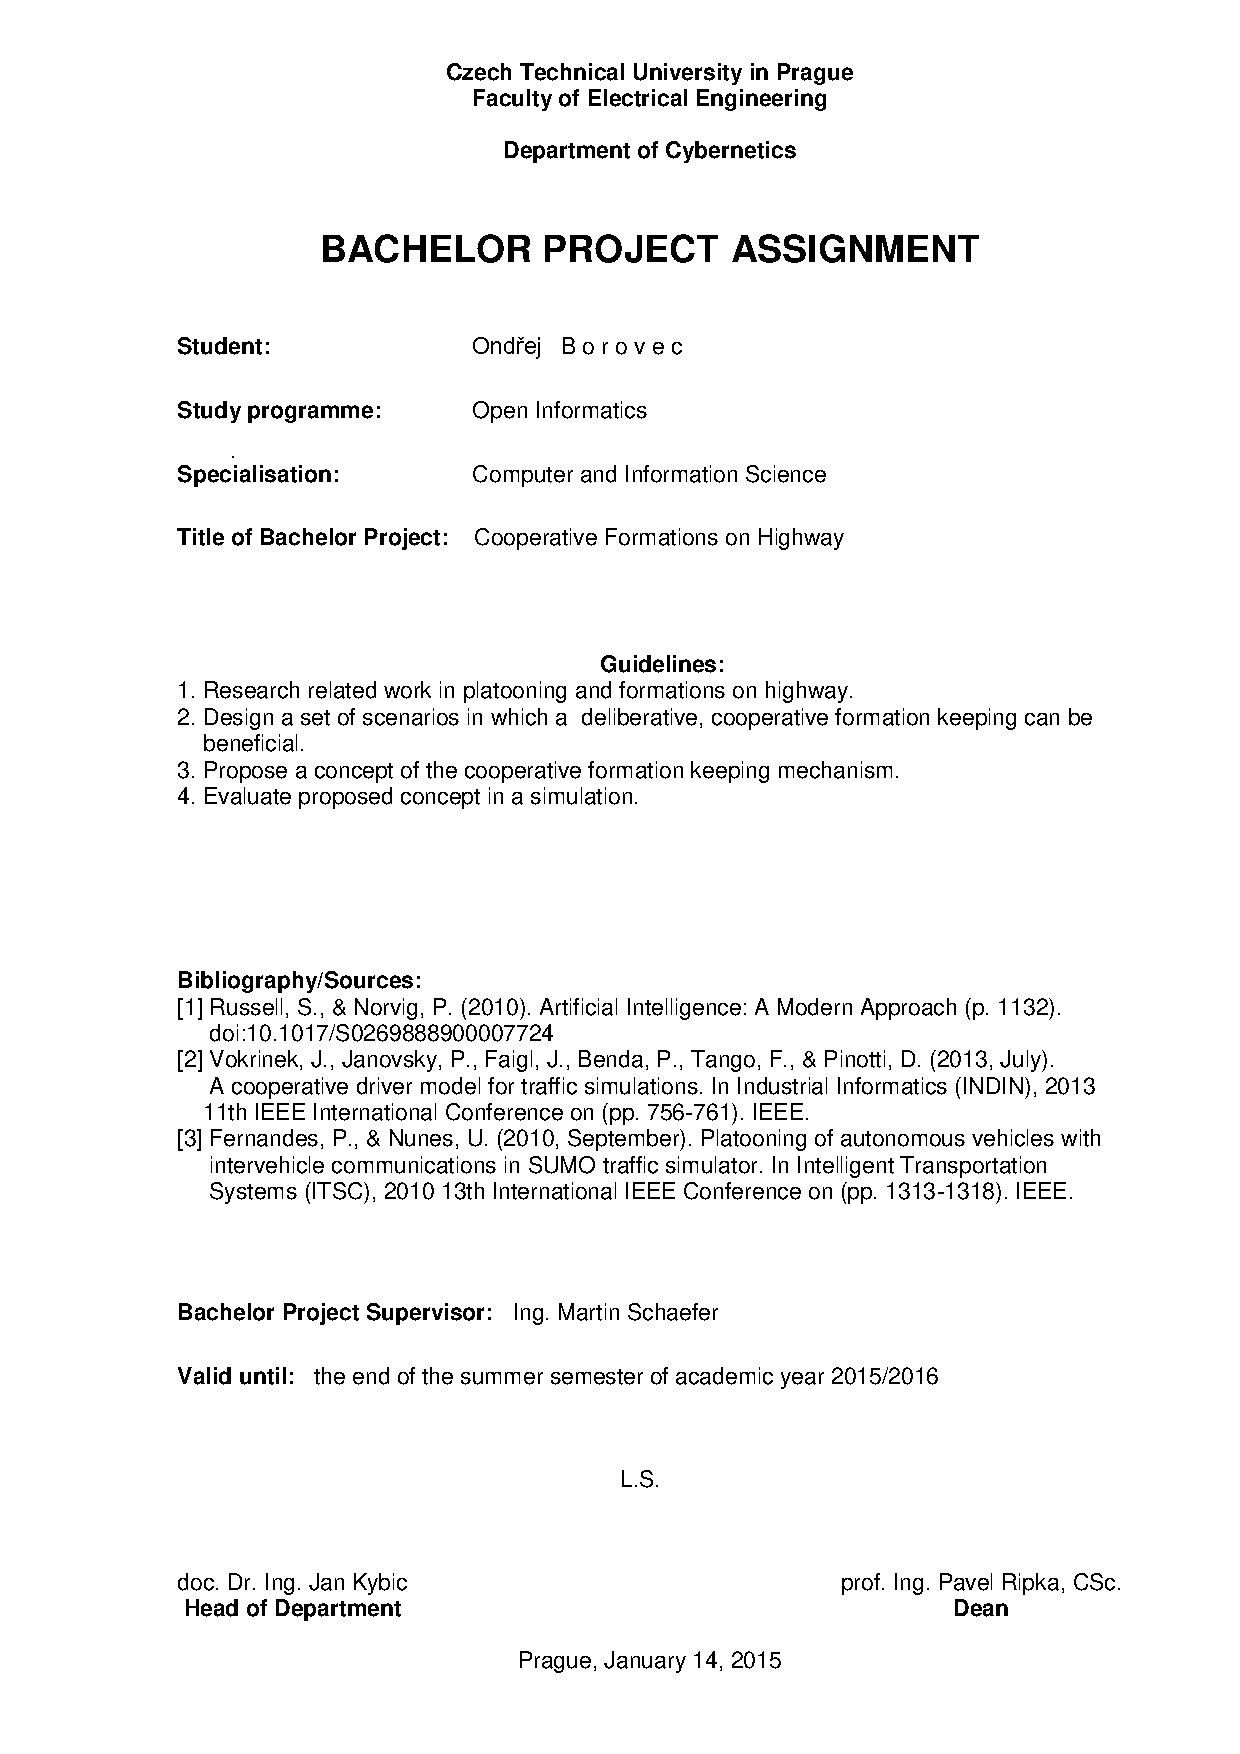
\includepdf[pages={1}]{ZadaniEng.pdf}

\includepdf[pages={1}]{blankPage.pdf}
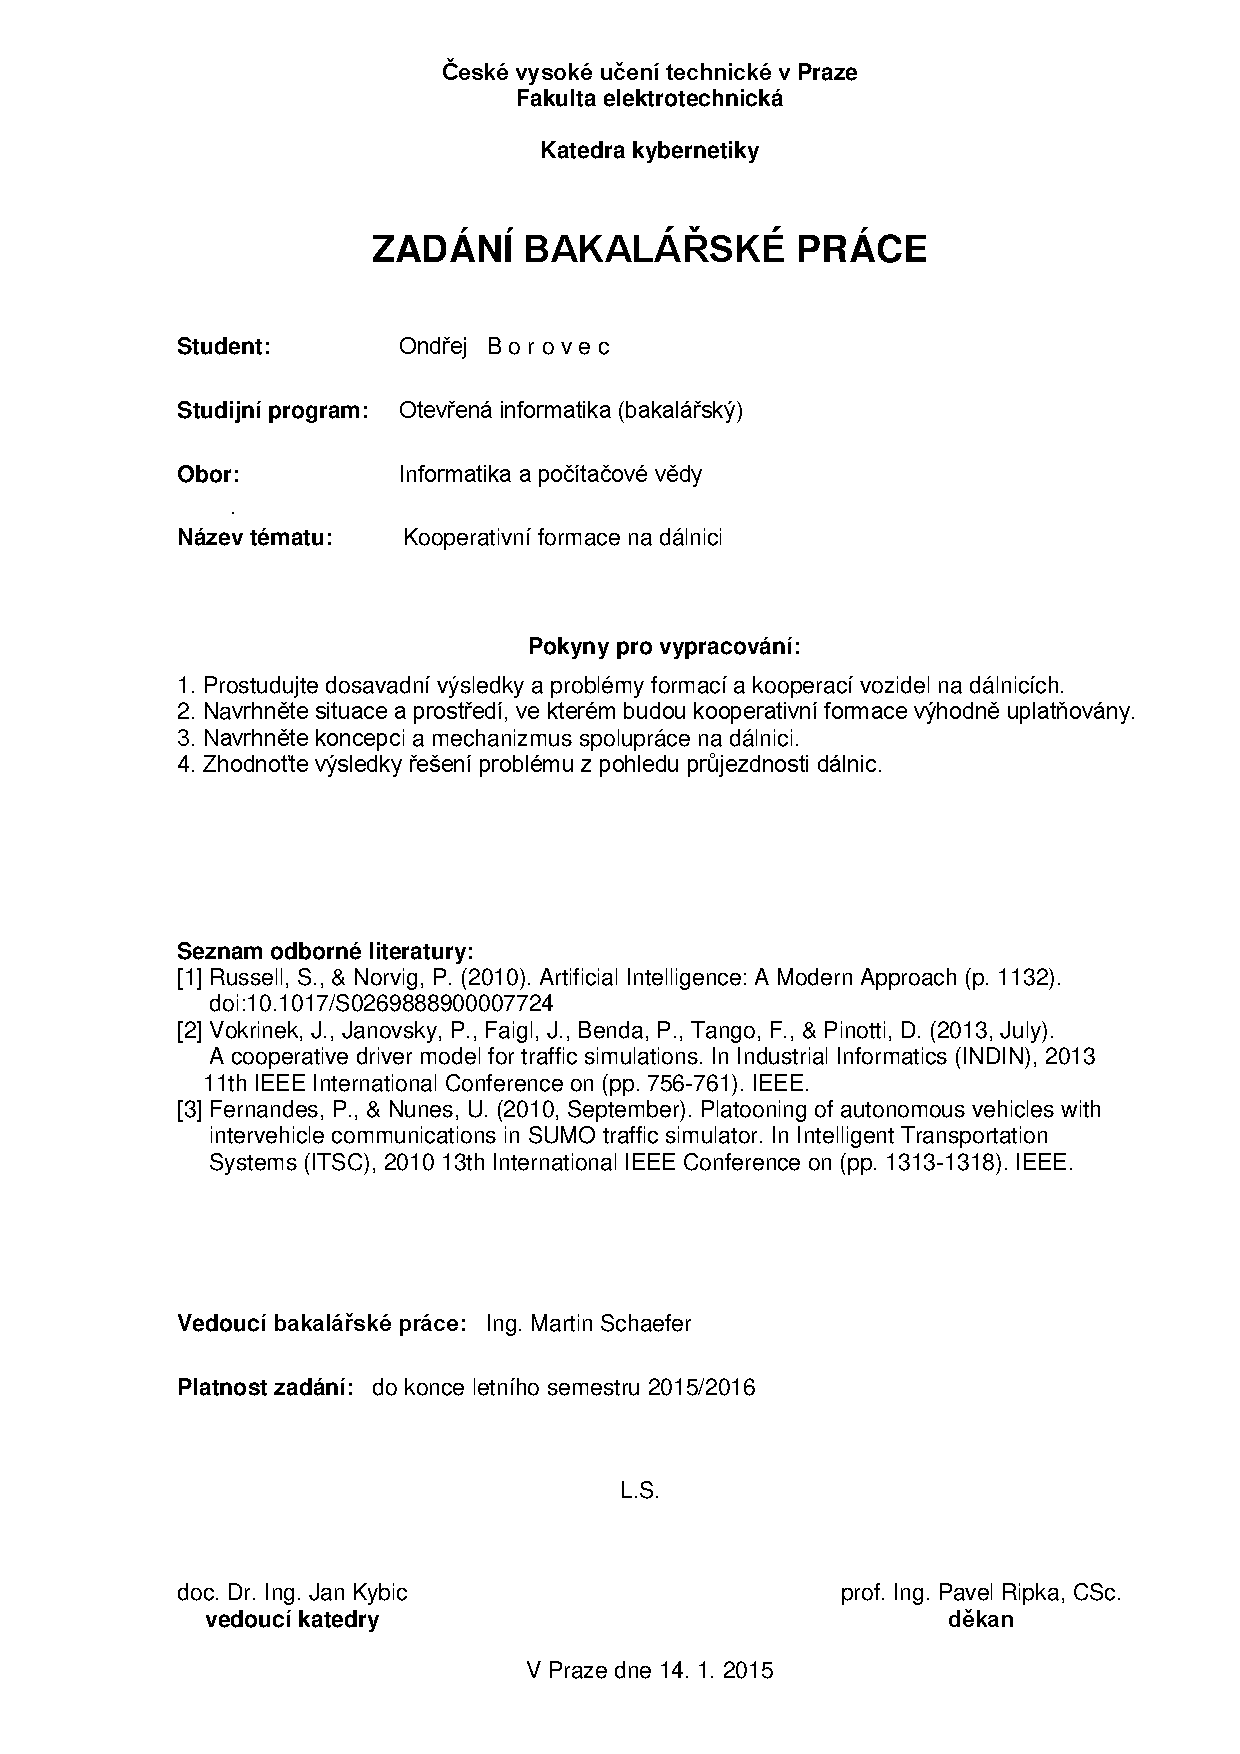
\includepdf[pages={1}]{ZadaniCz.pdf}
%%%%%%%%%%%%%%%%%%%%%%%%%%%    Podekovani / Acknowledgements 

\acknowledgements
\noindent
I wish to express my sincere thanks to Martin Schaefer for patient leading, my parents for helping me to improve English side of the thesis and SG-1 for supporting me during writing.


%%%%%%%%%%%%%%%%%%%%%%%%%%%   Prohlaseni / Declaration 


%%%\declaration{In Prague on May 25, 2015}

\declaration{V Praze 22. května 2015}


%%%%%%%%%%%%%%%%%%%%%%%%%%%%    Abstract 
 
\abstractpage

This thesis deals with advantages and the effect of platooning concept on highway traffic both in general sense and for the structure of traffic in the Czech Republic. Three different approaches to the cooperation of the vehicles in the platoon during changing of lanes were studied and described and they were compared in terms of safety of traffic, reached maximum capacity of highway and average speed of passenger vehicles. In order to realize the simulations, the traffic simulator Alite has been improved and a module that supports "platooning" concept has been developed. The simulated environment is based on a simple basic statistical analysis of highway data and the results of simulation were validated by comparison with theoretical assumptions and results. 

We created two traffic models, that simulate traffic density of highway with real ration of passenger vehicles and trucks in rush hours. Their simulation results verified the assumption that "platooning" increases highway capacity and helps to increase the average speed. Other experiments proved, that cooperative platoons have small negative effect on these features, but platoons increase safety of changing of lane. Based on these results, we recommend applying platooning concept on with higher cooperation level.


\abstractpageCZ
Tato bakalářská práce se věnuje výhodám a efektu formací na dálniční dopravu jak v obecném pojetí, tak i pro strukturu dopravy České republiky. Byly prostudovány a detailněji popsány tři přístupy ke kooperaci vozidel ve formaci, které byly porovnány i z hlediska bezpečnosti, dosažené průjezdnosti a průměrné rychlosti osobních automobilů. Pro simulaci byl vylepšen dopravní simulátor Alite a vyvinut modul podporující formace vozidel. Vlastnosti simulovaného prostředí jsou založeny na jednoduché analýze statistických dálničních dat a výsledné hodnoty simulace byly ověřeny porovnáním s teoretickými předpoklady a výsledky. 

Byly vytvořeny dva dopravní scénáře simulující zatížení části dálnice s daným poměrem zastoupení osobních a těžkých vozidel v dopravních špičkách, jejichž výsledky ověřily předpoklad, že formace aut zvyšují maximální průjezdnost dálnic a zvyšují průměrnou rychlost při průjezdu. Dalšími experimenty bylo prokázáno, že mírně negativní efekt na tyto vlastnosti má vyšší stupeň kooperace formací aut, který ale zvyšuje celkovou bezpečnost přejíždění mezi pruhy. Na základě výsledků experimentů doporučujeme implementaci konceptu formací s vyšší spolupráci mezi jednotlivými vozidly.

\noindent


%%%%%%%%%%%%%%%%%%%%%%%%%%%%%%%%  Obsah / Table of Contents 

\tableofcontents


%%%%%%%%%%%%%%%%%%%%%%%%%%%%%%%  Seznam obrazku / List of Figures 

\listoffigures


%%%%%%%%%%%%%%%%%%%%%%%%%%%%%%%  Seznam tabulek / List of Tables

\listoftables


%**************************************************************

\mainbodystarts
% horizontalní mezera mezi dvema odstavci
%\parskip=5pt
%11.12.2008 parskip + tolerance
\normalfont
\parskip=0.2\baselineskip plus 0.2\baselineskip minus 0.1\baselineskip

% Odsazeni prvniho radku odstavce resi class book (neaplikuje se na prvni 
% odstavce kapitol, sekci, podsekci atd.) Viz usepackage{indentfirst}.
% Chcete-li selektivne zamezit odsazeni 1. radku nektereho odstavce,
% pouzijte prikaz \noindent.

%**************************************************************

% Pro snadnejsi praci s vetsimi texty je rozumne tyto rozdelit
% do samostatnych souboru nejlepe dle kapitol a tyto potom vkladat
% pomoci prikazu \include{jmeno_souboru.tex} nebo \include{jmeno_souboru}.
% Napr.:
% \include{1_uvod}
% \include{2_teorie}
% atd...

%*****************************************************************************


\chapter{Introduction}
Everybody is grateful for Karl Benz's invention which saved us a lot of time thanks to the possibility to travel by cars instead of by carriages. But since the time of Henry Ford, who started serial cars production, the number of vehicles on our roads has been constantly increasing, which brings new problems and issues. The first way, how to increase the capacity of roads was the concept of highways but nowadays the density of traffic on the highways has reached such a level of use that sometimes it is better to drive along side roads. At this time a lot of drivers, cars, passengers, goods all over the world are stacked  in traffic jams although it probably is not necessary. 

We reckon that there are some ways how to deal with this situation. We can build new transport environment such as much bigger highways and a totally new aboveground concept of transport. Or we can increase car and transport speeds. The maximum speed of most new vehicles is higher than 200 km/h, but the increase of transport speed is not the direction how people can save their time, because the driving speed is one of the most frequent reasons of car accidents \footnote{\url{http://www.drivers.com/article/1173/}}. There is also another way and it is an optimization of current traffic system, which could be much cheaper and the modification would be up to the customers not up to the government's decision.

From the computer science point of view, we can see vehicles as agents which can cooperate with each other. These more autonomous vehicles can have more levels of driver support such as helping the drivers by useful advice or having a total control over the vehicles. Fully controlled vehicles have the advantage that, program is deterministic so, it does not make mistakes and does not succumb to external influences and panic. The most discussed problem is the law aspect, who is responsible for mistakes caused by the “autonomous” drivers. 

The cooperation of vehicles using Vehicle to Vehicle (V2V) and Vehicle to Infrastructure (V2I) protocols is already well-known and there are already some examples of products of BMW\footnote{\url{http://www.motorauthority.com/news/1064910_bmw-shows-off-its-v2v-technology-with-5-new-videos}}, General Motors\footnote{\url{http://media.gm.com/media/us/en/gm/news.detail.html/content/Pages/news/us/en/2014/Sep/0907-its-overview.html}}, and Toyota\footnote{\url{http://www.toyota-global.com/innovation/intelligent_transport_systems/world_congress/2014detroit/pdf/ITS_Integrated_Safety.pdf}} which we can see in the streets (for example Advanced driver assistance system which helps you in complicated situations in city or collision detection). The limitation of these improvements is that not every car (mostly the old ones and low cost) can cooperate with these systems.

Based on research and papers published by many international projects, we would like to make some partial research, to extract rules and conditions for vehicle cooperation and platooning and  experiment with them.

In this thesis we focus on research about simulating platoon transport concept that can optimize traffic and increase the capacity of transport network. We also focus on its applicability to some of the Czech highway traffic structures. The situation and some traffic statistics of the Czech traffic system are in Chapter 2, with emphasis on the composition of the traffic and on current pass ability.  In Chapter 3 we did an overview of existent papers and projects and we set basic rules of platoon concept. Based on these rules we developed and customised a Traffic simulator for platooning on highway, which is described in Chapter 4. With this simulator we prepared some test scripts and simulated some cases with the platooning concept settings. The tests were designed from the point of view of maximum capacity of highways and of platooning effect on actual traffic structure and can be found in Chapter 5. We tested the efficiency of the platooning concept with different ratio of cooperating and non-cooperating vehicles. And in the last part we simulated the concept on real data from the Czech highways to support the decision whether the concept is valuable for the Czech environment. We also created a protocol for platoon overtaking and tested its positive effect in Chapter 6.

 

\chapter{Highway traffic in Czech Republic}

In order to be able to test platooning effects on real data of highway traffic in the Czech Republic we needed to take information about level of traffic statistics at different times in day and on different days in week, ration between passenger vehicles and trucks in highway, average speed and speed dispersion on highway. There is not a complex study which would provide us such information so we had to use some different resources and join them. We had to combine three sources of statistics and traffic models:

\begin{itemize}
\item Source 1:	Vysoké Mýto –  dopravní model a analýza dopravních proudů (Vysoke Myto – traffic model and analysis of traffic streams) Made by Moot MacDonald CZ, s.r.o. for Vysoke Myto council, published in January 2015\footnote{\url{http://projekty.vysoke-myto.cz/index.php/strategicke-dokumenty/dopravni-pruzkum}}.
\item Source 2:	Traffic statistics from tunnel Lochkov, Prague circuit – May 2014, received from ŘSD Praha – cannot be published
\item Source 3:	Traffic statistics of highway D1 published by ŘSD Praha in 2012\footnote{\url{http://www.ceskedalnice.cz/prilohy/intenzity-2012.pdf}}\footnote{\url{ttp://www.ceskedalnice.cz/odborne-info/intenzity-dopravy}}.
\end{itemize}










\section{Daily statistic and traffic structure }

The daily statistics are taken from Source 1 (Vysoke Myto) because it is a detail analysis. It was made on main route R35 that connects Bohemia and Moravia (Hradec Kralove – Olomouc) where there is no possibility to use a highway. All transit and local transport goes through this measured point and therefore the distributions of vehicle types and traffic density are similar to highway ones.


\begin{figure}[ph]
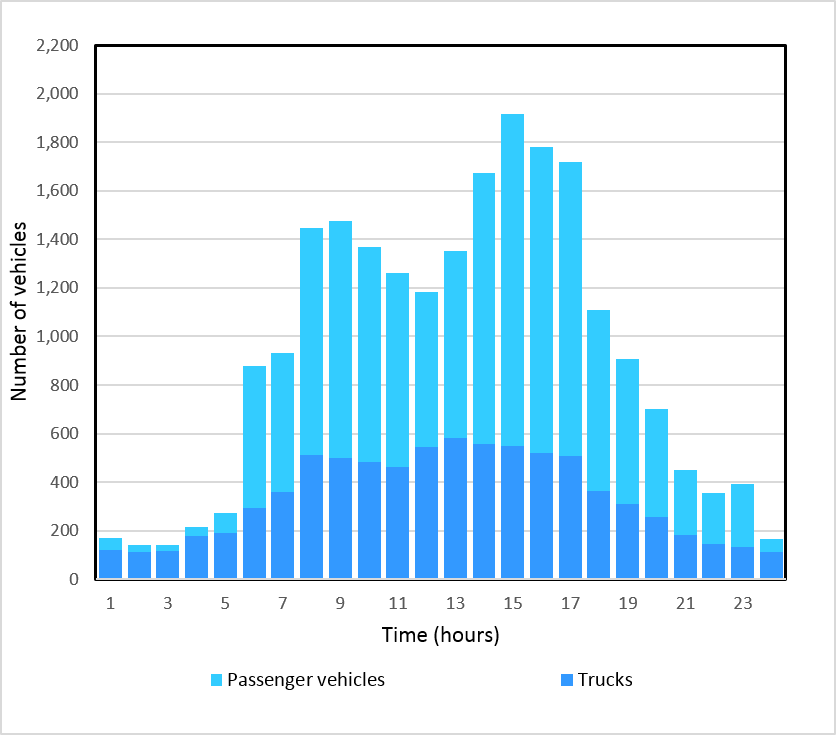
\includegraphics[width=0.90\textwidth,height=0.90\textheight,keepaspectratio]{figures/Chapter_2/2_Cum_diag_traffic_VM.png}
\centering
\protect\caption{\label{fig:2_1-1}Cumulative diagram of number of passenger vehicles plus number of trucks per hour during a day in Vysoke Myto}
\end{figure}

There are results of traffic monitoring which was made in Vysoke Myto in September 2014 in the Figure \ref{fig:2_1-1}. You can see that there are two  rush hours in a day (morning 7-10, 14-17 o'clock). The ratio passenger vehicles and trucks change in day, there are fewer cars in night hours and during day the number of cars increases and it is nearly double of trucks  as you can see in Table \ref{tab:2_1-1}.

\begin{table}
\begin{centering}
\begin{tabular}{|c|c|c|c|c|c|c|c|c|c|}
\hline 
Hours & 1:00 & 2:00 & 3:00 & 4:00 & 5:00 & 6:00 & 7:00 & 8:00  \tabularnewline
\hline 
Cars in traffic & 30\% & 21\% & 17\% & 16\% & 30\% & 67\% & 62\% & 65\%  \tabularnewline
\hline 
 &  &  &  &  &  &  &  &  \tabularnewline
\hline 
Hours & 9:00 & 10:00 & 11:00 & 12:00  & 13:00 & 14:00 & 15:00 & 16:00\tabularnewline
\hline 
Cars in traffic & 66\% & 65\% & 63\% & 54\% & 57\% & 67\% & 71\% & 71\%\tabularnewline
\hline 
 &  &  &  &  &  &  &  &  \tabularnewline
\hline 
Hours & 17:00 & 18:00 & 19:00 & 20:00 & 21:00 & 22:00 & 23:00 & 24:00\tabularnewline
\hline 
Cars in traffic & 70\% & 67\% & 66\% & 63\% & 59\% & 59\% & 66\% & 32\%\tabularnewline
\hline 
\end{tabular}
\centering
\protect\caption{\label{tab:2_1-1}Percentages of passenger vehicles in all traffic during a day}
\end{centering}
\end{table}

\section{Monthly statistic of cumulative quantity of vehicles}

For this statistic we decided to use Source 2 (tunnel Lochkov). In Figure \ref{fig:2_2-1} there is cumulative number of vehicles for both directions in May 2014. By this analysis we wanted to show, that the traffic distribution repeats  weekly and the level of traffic depends on working and weekend days.

\begin{figure}[ph]
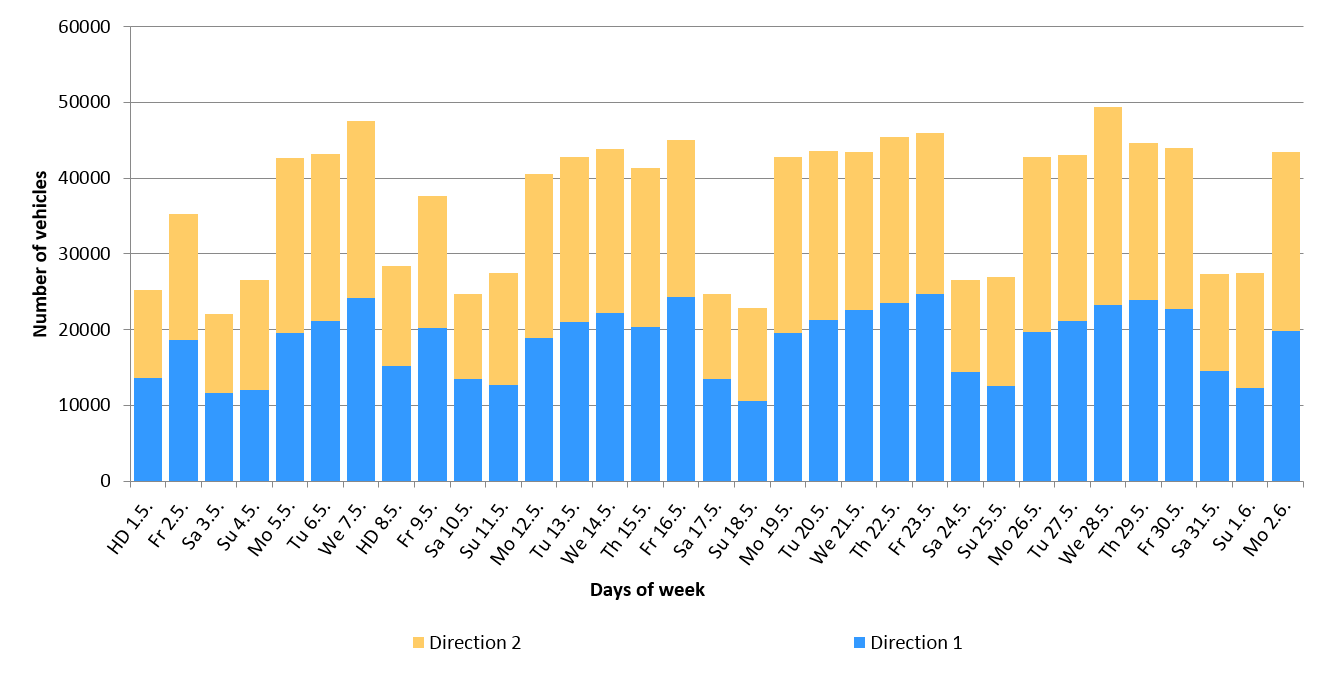
\includegraphics[width=0.85\textwidth,height=0.90\textheight,keepaspectratio]{figures/Chapter_2/2_Cum_diag_month.png}
\centering
\protect\caption{\label{fig:2_2-1}Cumulative diagram of number of traffic in both directions per day during May}
\end{figure}

In this monthly statistics (Figure \ref{fig:2_2-1}) you can see that traffic density is influenced by work days in week. On weekends the traffic density is about a half of work days density. In May 2014 there were two holidays during week (Thursday 1.5. and Thursday 8.5. in 2014) and you can see low traffic density too on these days, and even on the following Fridays the density is lower than on other Fridays.





  
  
  
  


\section{Number of vehicles per day in highway}

For this statistics we decided to use Source 3 (highway D1) where average number of vehicles per day is recorded in both directions in several parts of highway D1. See example in Table \ref{tab:2_3-1}. According to the data we can also say that in last several years there was no big increase of volume of traffic. So we can expect that the number of vehicles per day in year 2015 should be similar to the numbers in year 2012.

\begin{table}[ph]
\begin{centering}
\begin{tabular}{|c|c|c|c|c|c|c|}
\hline 
Part of D1 / Year & 1994 & 2000 & 2006 & 2008 & 2010 &  2012\tabularnewline
\hline 
Spořilov – Chodov & 47 700 &	71 400 &	94 900 &	98 200 &	88 800 &	90700\tabularnewline
\hline 
Chodov - Průhonice &	35 700 &	62 600 &	- &	91 900 &	82 500 &	84400\tabularnewline
\hline 
Soutice - Loket &	18 000 &	26 200 &	35 700 &	37 700 &	37 000 &	37000\tabularnewline
\hline 
Devět Křížu - Ostrov. &	20 400 &	35 800 &	39 100 &	41 300 &	41 200 &	41300\tabularnewline
\hline 
Ostrovačice - Kývadla &	20 900 &	36 700 &	39 900 &	- &	42 900 &	43100\tabularnewline
\hline 
\end{tabular}
\centering
\protect\caption{\label{tab:2_3-1}Number of vehicles which go though a part of highway D1 per day in both directions}
\end{centering}
\end{table}











\section{Speeds in highway}

For the maximum usage of highway it is expected to drive by maximum speed which is in the Czech Republic 130 km/h , it is about 36 m/s. For the simulator, Chapter 4, which increase the vehicle speed by 1 m/s in changing of lane, we set that average speed in 34 m/s. So in three-lane highway the average speed is not higher than speed limit.

We used speed dispersion of 3m/s to create various vehicles in highway, no two drivers go at the same speed.







\section{Model situations for simulation}

In order to make the future testing easier, we set some traffic model situations.


\subsection*{Traffic model \#1 – part of D1: Chodov – Průhonice}

This part of highway D1 was chosen as a three-lane highway which corresponds to classic example of highway entrance to a big city. We chose time 14:00 that is rush hour in highway and set modelling conditions in Table  \ref{tab:2_5_1-1} according Figure \ref{fig:2_5_1-1} for 42 200 vehicles per day (Table \ref{tab:2_3-1}) in one direction.

\begin{table}[ph]
\begin{centering}
\begin{tabular}{|c|c|}
\hline 
Number of vehicles per hour in one lane &	3 200\tabularnewline
\hline 
Average speed &	34 m/s\tabularnewline
\hline 
Speed dispersion &	3m/s\tabularnewline
\hline 
Percentage of passenger vehicles in traffic & 	67\%\tabularnewline
\hline 
Trucks speed &	25 m/s\tabularnewline
\hline 
Number of lanes in highway &	3\tabularnewline
\hline 
\end{tabular}
\centering
\protect\caption{\label{tab:2_5_1-1}Features of Traffic model \#1}
\end{centering}
\end{table}


\begin{figure}[ph]
\begin{centering}
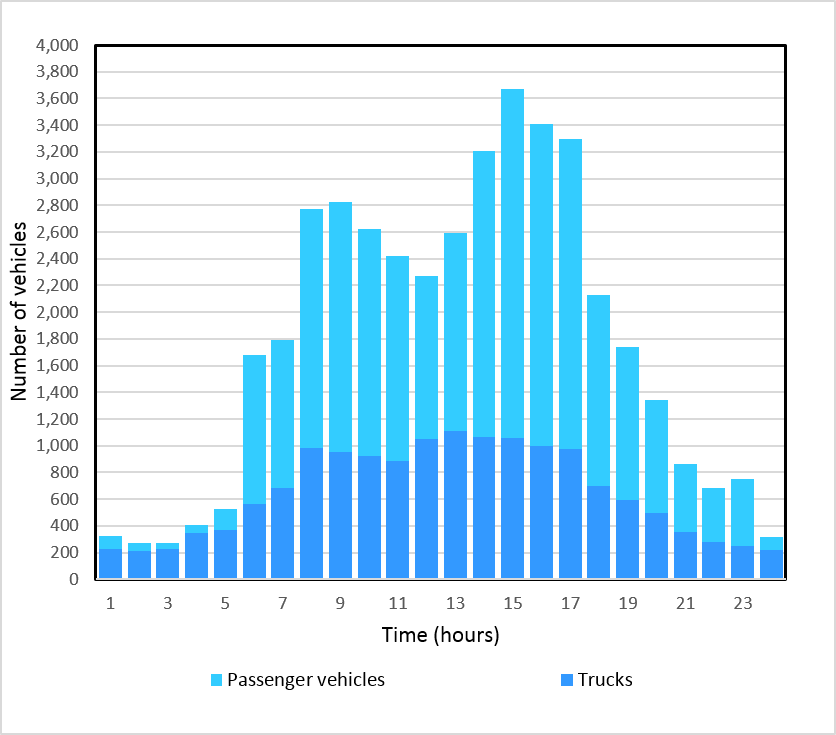
\includegraphics[width=0.60\textwidth,height=0.60\textheight,keepaspectratio]{figures/Chapter_2/2_Cum_diag_day_42200.png}
\centering
\protect\caption{\label{fig:2_5_1-1}Cumulative diagram of number of passenger vehicles plus number of trucks per hour for 42 200 vehicles per day}

\end{centering}
\end{figure}

\subsection*{Traffic model \#2 – Tunnel Lochkov}

We chose time 13:00 that is rush hour in highway (we wanted to test different than in Traffic model \#1) and set modelling conditions in Table  \ref{tab:2_5_2-1} according Figure \ref{fig:2_5_2-1} for 22 000 (average of workdays from Figure \ref{fig:2_2-1}) in one direction.

\begin{table}[ph]
\begin{centering}
\begin{tabular}{|c|c|}
\hline 
Number of vehicles per hour in one lane &	1 650\tabularnewline
\hline 
Average speed &	34 m/s\tabularnewline
\hline 
Speed dispersion &	3m/s\tabularnewline
\hline 
Percentage of passenger vehicles in traffic & 	67\%\tabularnewline
\hline 
Trucks speed &	25 m/s\tabularnewline
\hline 
Number of lanes in highway &	2\tabularnewline
\hline 
\end{tabular}
\centering
\protect\caption{\label{tab:2_5_2-1}Features of Traffic model \#2}
\end{centering}
\end{table}

\begin{figure}[ph]
\centering
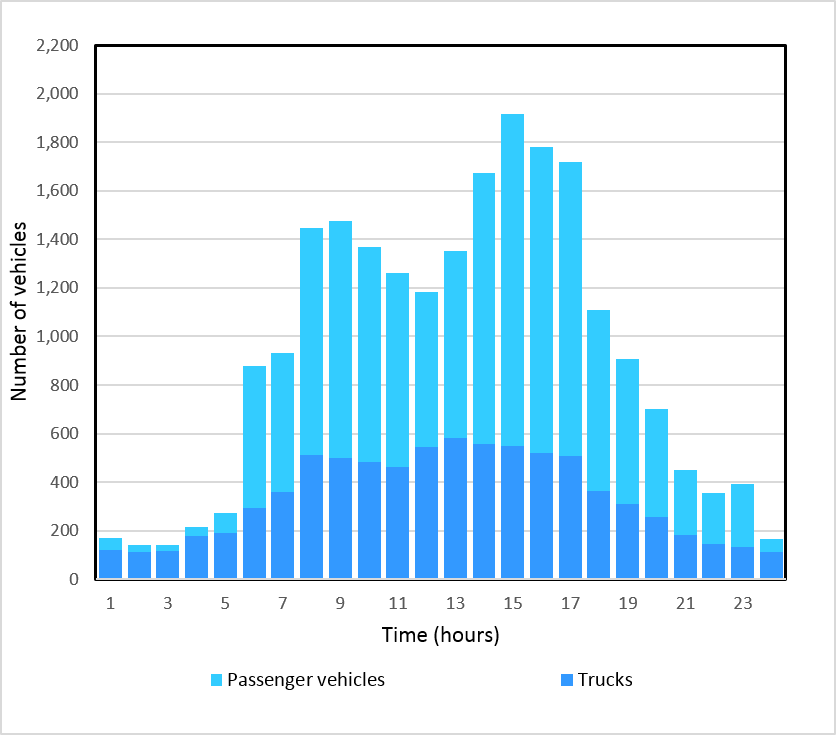
\includegraphics[width=0.60\textwidth,height=0.60\textheight,keepaspectratio]{figures/Chapter_2/2_Cum_diag_day_22000.png}
\centering
\protect\caption{\label{fig:2_5_2-1}Cumulative diagram of number of passenger vehicles plus number of trucks per hour for 22 200 vehicles per day}
\end{figure} 

\newtheorem{theorem}{Theorem}[section]
\newtheorem{corollary}{Corollary}
\chapter{Platooning}
The first idea of platooning was published in \cite{shladover1979} with the definition:

\textit{
\newline
Platoon is a collection of vehicles that travel close together, actively coordinated in formation.}
\newline

But this formulation is not as specific as it would be for our situation, so we prefer the definition which is mentioned in SARTRE platooning concept \cite{bergenhem2010challenges}:

\textit{
\newline
A platoon is a number of vehicles that are travelling together and electronically connected. There is one lead vehicle and one or more following vehicles. The following vehicles of a platoon are controlled autonomously while the lead vehicle is controlled manually}
\newline

As it is mentioned in the previous definition, the biggest interest in platooning appeared with the development of electronic communication channels - Vehicle to Vehicle (V2V) and Vehicle to Infrastructure (V2I) based on wireless connection.

This idea enchanted a lot of people all over the world and now there are several projects which are working on this topic. The most known are SARTRE\footnote{\url{http://www.sartre-project.eu/en/Sidor/default.aspx}}  (Europe), PATH\footnote{\url{http://www.path.berkeley.edu/research/automated-and-connected-vehicles/truck-platooning}}  (USA), GCDC\footnote{\url{https://gcdc.net}}  (Germany), SCANIA\footnote{\url{http://www.scania.com}}  (Europa - Japan), Energy ITS\footnote{\url{http://orfe.princeton.edu/~alaink/SmartDrivingCars/ITFVHA13/ITFVHA13_JP_Energy_ITS_Tsugawa.pdf}}  (Japan), AUTO21\footnote{\url{https://www.auto21.ca/en/}}  (Canada) and many others. These projects cannot be described together because they differ in specific parts, but all of them are proving positive effects of platooning concept on highway traffic.

\newpage
\section{Recent research projects overview}

International Europe project SARTRE - Safe Road Trains for the Environment is funded by the European Commission and includes many European science and university institutes and it also cooperates with Volvo research centres. It is a complex solution which includes longitudinal and lateral control of platoons of both types of vehicles (heavy vehicles trucks and passenger vehicles - cars). Vehicles communicate with each other only via V2V communication channel based on ITS-G5 and it means, no changes in highway infrastructure are necessary. Another project which is suitable for mixture of passenger vehicles and trucks is project GCDC, Grand Cooperative Driving Challenge in Germany, which is implementable in urban environment too.

Another group of projects is focused only on trucks. One of such projects is SCANIA in which they are working on safety longitudinal control (lateral movement is manual) without any change on routes. Project Energy ITS is one of the most recent projects which started in 2008. To compare it with the previous one, trucks have automatically a lateral control too, but it assumes lane markings in highway. Very similar to those projects is German KONVOI\footnote{\url{https://www.ika.rwth-aachen.de/pdf_eb/gb6-24e_konvoi.pdf}}  too.

The California (Berkeley) project PATH - Partners for Advanced Transportation Technology belongs into the special category. Its idea allows platooning of passenger vehicles or trucks, these two types of vehicles cannot be mixed. It assumes dedicated lanes with embedded reference markers in the road surface and with this condition the vehicles are able to do longitudinal and lateral control. The most interesting thing and what is totally different from other projects is that even the leading car is fully autonomously controlled.

\section{Lifecycle of platoon}

The concept of platooning has three main lifecycle sections of a platoon. The first section is how the platoon should be created and how to sort vehicles in a platoon, in a convoy. The second section is a task about acting and behaviour on highway and the last section is about leaving the platoon. This thesis is focused on the second one (behaviour) and simulates and analyses the vehicle and platoon behaviour in highway traffic. Below there is a description of all parts of the platoon lifecycle for better understanding of these topics.

\subsection{Formation of platoon}

Every highway entrance ramp or highway entrance ramp lane is a point of decision, which platoon the vehicle will be assigned to, or whether the vehicle will create its own platoon of which it will be the lead vehicle. This decision is based on thresholds how much the vehicle would have to change its speed and what distance is to some already existent platoons driving on highway. 

This part is also important for sorting of vehicles, because only here we can actively manage the order of vehicles in platoons. According to most recent projects – see in references, every vehicle in platoon should be in the order in which they leave the highway and the platoon. It means the last vehicle in the platoon will leave the platoon and the highway as the first  vehicle.

If a vehicle wants to join an existent platoon, other vehicles should create space behind the platoon or the platoon vehicles should create space inside the platoon to provide right position order inside the platoon for the new vehicle.

\subsection{Platoon behaviour on highway}

This part of the platoon lifecycle describes the period between establishing and decomposition of platoon, the period between entering and leaving of the vehicle into or from the platoon; it means that the platoon is moving without changing the numbers of vehicles in the platoon. Changes of platoon content or order are considered as decomposition and establishing of platoon. During this lifecycle period the platoon solves several partial problems, for example how to behave during overtaking, changing of lane, changing of platoon speed and distances between platoon vehicles, etc. or what to do with “problematic” drivers who try to destroy the cooperation of the vehicles that are included in the existent platoon. This second mentioned problem can be solved by changing the distances between the vehicles in the platoon, i.e. reducing the distances so that not “to allow” the other vehicles to get into the platoon and “to destroy” it.

This state, going/being in platoon, is the biggest part of driving on the highway. In this state the vehicles of the platoon stay for most of their time on the highway. So it is not a surprise that most of the optimization must be done there. The distance between the vehicles in the platoon and also the maximum number of vehicles which can be in one platoon have the main influence and are very important for the increase of traffic capacity.

\subsection{Decomposition of platoon}

Leaving the platoon should be the easiest part of platoon lifecycles because at this time the leaving vehicle should be on the last position in the platoon order. So the vehicle only slows down and leaves the platoon and later also the highway or goes into another platoon.

\section{Advantages of platoonig concept}

The main reason of platoon research on highway is to increase lane traffic capacity. It means that more vehicles can pass through a part of highway per a time period, the most common indicator “capacity of lane” is the number of vehicles per hour. So the equation for maximum safety capacity is: 

\begin{equation}\protect\label{eq:max_cap_single}
c_{max}=\frac{3600}{s+t_{s}\cdot v}\cdot v
\end{equation}

where  $c_{max}$  is the maximum capacity of vehicles per lane and per hour to steady state speed $v$ in meters per second, $s$ is the average length of a vehicle in meters and  $t_{s}$ is the time between two vehicles (safety time) in seconds.

For the calculation of maximum capacity of lane with platoons, we have to change the equation into the form which includes more parameters, but it is only a generalization of the Equation \ref{eq:max_cap_single}:

\begin{equation}\label{eq:max_cap_platooning}
c_{max}=\frac{3600\cdot X}{(X-1)\cdot(d+s)+s+t_{s}\cdot v}\cdot v
\end{equation}

where $X$ is the maximum number of vehicles which can be in one platoon and $d$ is the distance between two vehicles of the platoon in meters, distance between vehicles in platoon is constant. It assumes that distance $d$ is a constant for all speed of platoon so there is a space for more optimization but for this thesis this Equation \ref{eq:max_cap_platooning} is sufficient. We can also see that Equation \ref{eq:max_cap_platooning} is the same as Equation \ref{eq:max_cap_single} for  $X=$ 1  which means, platoons consist of one vehicle. Similar equation was published in \cite{dao2013strategy}, but we had to adapt it for our purposes. 

There is a "rule" for safety driving on highways in the Czech Republic which says that there should be a safe distance between two vehicles of the same speed which corresponds to the distance travelled by car for a period of 2 seconds. This is not an official rule, but it is a recommendation given in every driving school.

Let us assume an example with one highway lane in which there is an average speed \mbox{$v$ = 108 km/h} which equals to 30 m/s. Let us set other parameters: \mbox{$t_{s}$  = 2 s} (which corresponds to the recommended safety time in the Czech Republic), \mbox{$s$ = 4 m}, \mbox{$X$ = 5} and \mbox{$d$ = 6 m}. With these conditions the maximum capacity  $c_{max}$   of the highway without platooning concept \mbox{($X$ = 1)} will be 1 687 vehicles per hour and on the other hand the vehicles capable of platooning increase the maximum capacity $c_{max}$ to 5 400 vehicles per hour. This example proves a positive impact of platooning on maximum highway capacity because in optimal conditions platoons of 5 vehicles increase the capacity more than 3 times.

In the following Figure \ref{fig:3_3-1} you can see dependency of average speed in a lane and maximum capacity in the lane for cooperative and non-cooperative vehicles. The rest of variables are the same as in the previous example.

\begin{figure}[!htbp]
\centering
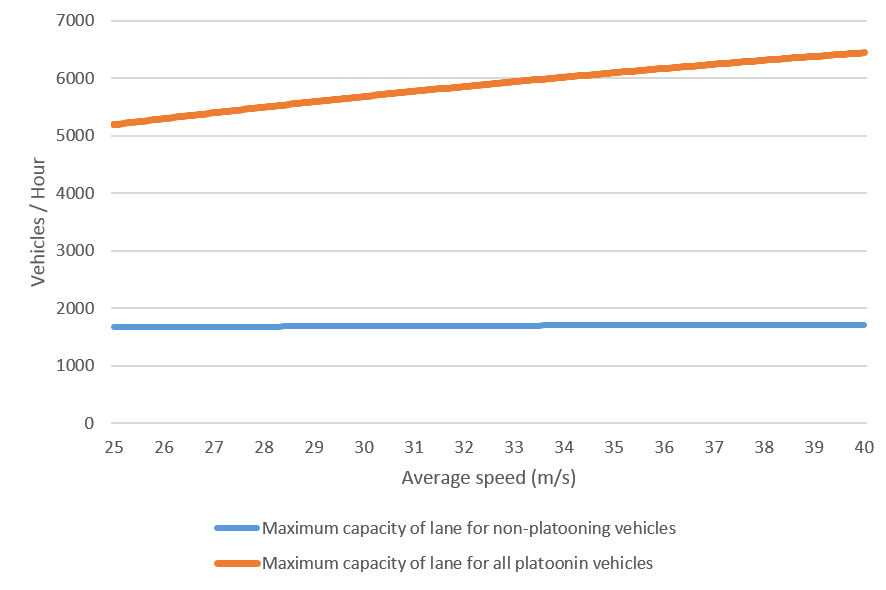
\includegraphics[width=0.90\textwidth,height=0.90\textheight,keepaspectratio]{figures/Chapter_3/3_curve_nonXplatooning_vehicles.png}
\centering
\protect\caption{\label{fig:3_3-1}Maximum capacity of lane for different average speeds}
\end{figure}

The increased capacity of highway is not the only positive effect of this concept. Autonomously controlled vehicles can also help with traffic safety, because of V2V communication, the vehicles can have on-line information about problematic situations and risks, they can react faster and therefore they have a longer time to solve the situation. In case that all vehicles can cooperate together, they can share information  e.g.. about braking and a vehicle can slow down faster than its driver can notice the action.

Another positive result of platooning and its close formation is the possibility to save fuel. Browand and Michaclian\cite{zabat1995estimates}\cite{browand2000platoon} proved that in the platoon of speed 96km/h with distance between vehicles 3 m, every vehicle (except for the leading one) can save from 5\% to 12\% of fuel depending on the type of vehicles. As an additional austerity result of this approach, it also decreases the amount of emission of $CO_{2}$ up to 2\%

\section{Disadvantages of platooning concept}

Concept of platooning is based on autonomous controlled vehicles, so there is a problem of responsibility for accidents which are caused by not human control. But this issue is not a matter of this thesis. Another problem is different level of driver’s knowledge and experiences. The first driver has to do the hardest work, because he has to lead the platoon  although he has no benefit of fuel savings. In agents technologies, this problem is called unfairness.

\section{Platoon rules}

In this part we describe the platooning concept which will be used in this thesis. The platoon consists of vehicles (up to maximum number) and “only” the first one is controlled by human driver, let us call the vehicle as Lead vehicle (LV). LV is equipped with some kind of driving assistant which helps to the driver and with an emergency assistant which can take control during emergency situations. So such a vehicle driver should have better driving skills. The rest of the vehicles are called Following Vehicles (FV) and they could be controlled automatically. Example of platoon you can see in next Figure \ref{fig:3_5-1}.

\begin{figure}[!htpb]
\centering
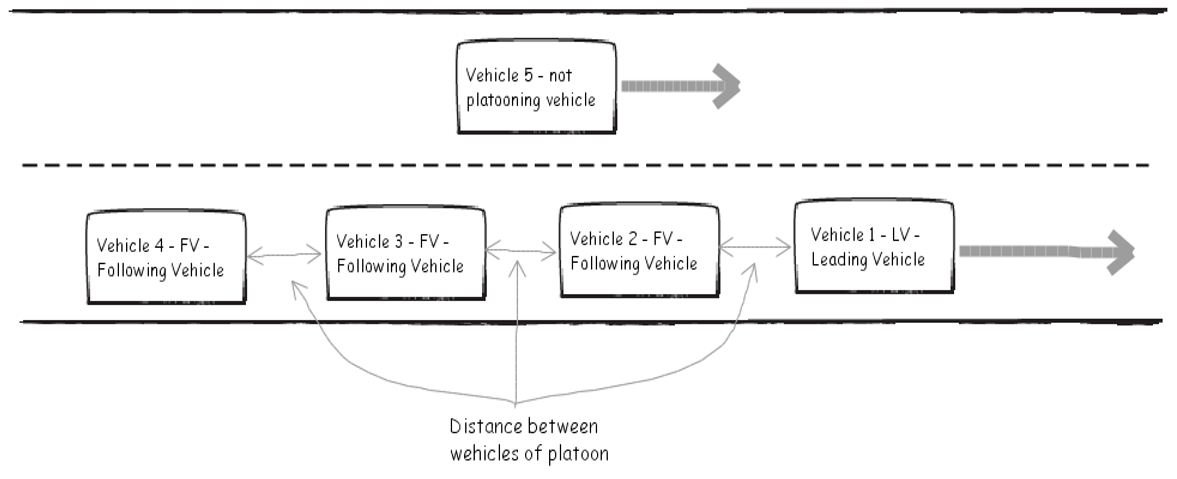
\includegraphics[width=0.90\textwidth,height=0.90\textheight,keepaspectratio]{figures/Chapter_3/3_platoonin_example.png}
\centering
\protect\caption{\label{fig:3_5-1}Example of structure of platoon of 4 vehicles}
\end{figure}

Each vehicle that is able to cooperate is equipped with V2V communication equipment and radar which provides information about all vehicles in reasonable range. So every platoon vehicle can check whether the neighbour lane is free to move there or whether the LV is in safe distance to the vehicle which is in front of it.

Every platoon has its constant preferred speed which can be increased only in case of overtaking a vehicle the speed of which is very similar to the speed of the platoon. This can be done so as not to block the faster lane for a long time. The platoon also changes its speed in problem situations such as traffic jam or traffic accident.

Every auto-controlled FV keeps distance at least 5 m to the front vehicle, but the distance can be changed for some operation of the platoon. For more safety the safe distance time of LV could be increased from 2s to 3s because in case of a collision of LV, every FV will have the collision too (it is not implemented in our simulator). 

\chapter{Traffic simulator}

We created a traffic simulator for the testing of platooning concept and cooperation of vehicles in platoons. For verification and testing of our assumptions and theories we had to set up a simulation environment which tries to compare real traffic transport statistics with general driver’s behaviour. We did not find an adequate simulator which would satisfy our needs (response time, flexibility, user modifiability, customisability), so we had to create a new one. In this part we will describe our used simulation environment and its features which affected our tests. 

For creation of multi-agent simulation scenarios we use and customize the simulation toolkit Alite that is also used for some projects inside AgentDrive platform developed by Agent Technology Centre in CTU.





\section{Alite and AgentDrive platform simulations}

The Alite is an agent-based simulation toolkit for multi-agent systems which corresponds to our need for big traffic simulation of independent vehicles. All description of project Alite can be found on its websites\footnote{\url{http://jones.felk.cvut.cz/redmine/projects/alite/wiki/Alite_Overview}}\cite{schaefer2011}.

The original composition of AgentDrive (which is based on Alite simulator) simulation mostly consists of two parts which have event based communication. The main part of the program – Highway module - contains all data of simulation and agents and it sends events and data into the second part - Simulator Lite - where graphical visualization is realized and physical simulation is also done. The Simulator Lite sends back the information about the actually changed positions of all objects depending on the physical aspects such as acceleration or maximum steering angle and so on. 

The agents then react on the changed positions and Highway module again sends new agent’s actions into simulator, such as the way-point where the adequate object (agent vehicle) should go. In the base implementation there was only an agent called RouteAgent which was able to follow its way and slow down in curves but it was not able to react to other agents.

\section{Our main improvements}

In source code of used simulator we had to do several changes with the graphical visualisation routines of highway simulation module to be able to realise and verify our assumptions. In this chapter there are descriptions of the main modifications to which we refer in next chapters and which set basic features of our highway simulator.

Since we use a big amount of vehicles (thousands of units), we decided not to use graphical visualisation of Simulator Lite , but to use only simulation functions of Simulator Lite and to use default visualisation in  Highway module. In Simulator Lite some time delays appeared in comparison with real time, because of compression and decompression of big quantity of commands. We could omit the physical model, because we assume straight or slightly curved highways and acceleration and deceleration of cars is included in vehicle-agent behaviour. 

We also add a possibility to define and simulate passenger vehicles (cars) and trucks, two main types of traffic participants. These two types are different in length and have several different characteristics. The speed of the cars is various according to the car speed Gaussian distribution, but trucks use defined limit speed and both the vehicle types have also a little different behaviour (see more details in next chapters).

\subsection{Java class: PlatooningAgent}

PlatooningAgent is derived from default RouteAgent which only follows generated predefined way-points. The instance holds basic information about the agent as a vehicle, it has different braking acceleration coefficients for dry, wet and snowy weather as well as information about index of lane in which the agent is.  We also added next abilities and features: 

\begin{itemize}
\item Counting Breaking coefficient - This feature returns breaking coefficient according to defined safety conditions.
\item Speeding up, acceleration – Agent can increase its actual speed up to its defined maximum value. The speed growth is directly proportional to the acceleration time. At this moment we use the same coefficient for acceleration and deceleration depends on safety conditions.
\item Slowing down, deceleration – It is very similar to Speeding up feature, but in opposite direction, value is going down to the limit 0 m/s.
\item Changing lanes – this function actively controls changing of lanes.  
\end{itemize}

\subsection{Java class: VehicleGenerationModule}

It could be expected that the Module generates vehicles only in the right highway lane and into the left lane the vehicle moves by overtaking and changing of lane, as it is usual by standard driver’s behaviour after the car is starting on highway by using a highway entrance ramp lane. But it is not true for our traffic simulator scenarios, because we simulate an existing traffic, so the Module generates agents in each  lane (according to vehicle type), even in the left lane.

This module works as the statistic centre for generation of new vehicles, it does not create new agents. According to statistic data it provides information whether a new vehicle should be generated there or not. It reads next entry parameters from platooning.groovy configuration file, in section platooning.VehiclesGenerationModule:

\begin{itemize}
\item	\textit{Generation limit} [Boolean] – Parameter decides either to use the Total number of vehicle per hour limit parameter or to generate as many vehicles as it is possible, it means to  generate another vehicle every time if  there is enough space to position it on highway.
\item	\textit{Total number of vehicles per hour} [Integer] - It is a maximum number of vehicles which should be generated in one hour in case there is enough space to generate them. Other vehicles can be added only if the ratio of total number of generated vehicles and time from the start of simulation is lower than this parameter.  
\item \textit{Passenger vehicle ratio} [Float] – Necessary only if value Simulator Lite \textit{Generate trucks} is true. It is number between 0 and 1 which corresponds to the percentage of passenger vehicles in  the number of all generated vehicles.
\item \textit{Average speed and Speed dispersion} [Float] – by these two parameters the speed Gaussian distribution of cars on highway is influenced.
\item \textit{Minimum speed} [Float] – Minimum vehicle speed limit is set.
\item \textit{Ratio of platoon vehicles} [Float] – Number from interval 0 to 1 which corresponds to how many percent of passenger vehicles should be placed in platoons.
\item \textit{Maximum length of platoon} [Integer] – Corresponds to maximum number of following vehicles in platoon. VehiclesGenerationModule generates platoons with number of following vehicles by Uniform distribution from 2 to this parameter.
\item \textit{Generate trucks} [Boolean]– This parameter decides whether to add or not a trucks to the simulation.
\item \textit{Truck speed} [Boolean] – It is a speed that is common for all generated trucks.
\end{itemize}


It is possible to set up these parameters variously , but for realistic simulation it is recommended to see Chapter 2.




\subsection{Java class: PlatooningCenterModule}

This obejct is responsible for traffic safety, it also contains all main platooning logic and agents’ decisions. We decided to centralize all logic and variant decisions into this location instead of to the agent class, because then it is easier to do changes and to debug the progress. After the platooning concept is finished, the concept can be easily moved to PlatooningAgent class.

This class is responsible for adding new vehicles into simulation, for changing of speed and lane of agents and for printing statistic information into external file for subsequent evaluation. 

\subsubsection{Passenger vehicles and trucks}

PlatooningCentreModule adds passenger vehicles or trucks according to information from VehicleGenerationModule. All vehicles (cars and trucks) can be formed now into platoons (in the past it was possible only with cars). They have their own \textit{Preferred speed}. It means that each vehicle has its own speed that it prefers to drive and its actual speed equals to this \textit{Preferred speed} or it is lower. 

Both types of vehicles (cars and trucks) differ in some of their properties.

Passenger vehicle:

\begin{itemize}
\item \textit{Preferred speed} of agent is generated in VehicleGenerationModule according to the Gaussian distribution influenced by parameters \textit{Average speed} and \textit{Speed dispersion}, agents have different \textit{Preferred speed}.
\item Agent can be generated and starts in every lane.
\item Agent can change lanes during simulation.
\end{itemize}

Truck:

\begin{itemize}
\item \textit{Preferred speed} of agent equals to parameter \textit{Truck speed}, all truck agents have the same \textit{Preferred speed}
\item Agent can be generated and starts only in right lane.
\item Agent cannot change lane during simulation
\end{itemize}

\subsubsection{Distance conditions}

In order to make the traffic in simulator safety, we set up some rules which are based on following definitions:

\begin{itemize}
\item \textit{Reaction distance} – $s_r$ – Distance that a vehicle travels during simulator response time (it waits for simulator back event). This distance would be important especially for simulator with high response time.

For $t_{sim}$ is run time period of simulator, that is defined as 0.1 second, and $v$ is speed of vehicle

\begin{equation}
s_{r}=t_{sim}\cdot v\label{eq:sr}
\end{equation}

\item \textit{Safe time distance} - $s_{std}$ -  it corresponds to distance which vehicle travelled over Safe time by its speed. Safe time\footnote{\url{https://www.gov.uk/general-rules-all-drivers-riders-103-to-158/control-of-the-vehicle-117-to-126}} – $t_{s}$ is a recommended time which should be between two vehicles going at the same speed, so the back driver is able to react a dangerous distance to the front car. Minimal recommended value is 2 seconds (you can also find it as “2 second rule”). Safe time is set in our simulator to 2 seconds too. We select this minimal value, because we would like to maximize  the highway traffic. For vehicle speed $v$:

\begin{equation}
s_{std}=t_{s}\cdot v=2\cdot v\label{eq:std}
\end{equation}

\item \textit{Slow down distance} – $s_{sdd}$ – Distance which is needed to slow down the back vehicle to the speed of the vehicle going ahead. When the front vehicle is faster than the back one, this distance is equal to zero.

For back vehicle speed $v_b$, front vehicle’s speed $v_f$ and deceleration $a_b$ of back vehicle:

\begin{equation}
v_{b}>v_{f\:}:\:s_{sdd}=\frac{v_{b}\cdot(v_{b}-v_{f})}{a_{b}}-\frac{0.5\cdot(v_{b}-v_{f})^{2}}{a_{b}}\label{eq:ssdd}
\end{equation}

\item \textit{Different speed correction} - $c_{ds}$ – is a value that corresponds to quadrat of difference of back vehicle speed and front vehicle speed. This value can equal maximally to 40\% (we used this value for the thesis, but it can be set in setting file of simulator) for this thesis of \textit{Safe time distance} of the back vehicle. The correction serves as an indicator of how much can a vehicles disrupt a \textit{Front safe distance} (described lower) of a overtaken vehicle.

For the back vehicle speed - $v_b$, the front vehicle speed $v_f$, back vehicle \textit{Safe time distance} - $s_{stdb}$:

\begin{equation}
c_{ds}=min(0.4\cdot s_{stdb},\frac{(v_{f}-v_{b})^{2}}{min(v_{f},v_{b})}\cdot s_{stdb})\label{eq:cds}
\end{equation}

\end{itemize}

\subsubsection{Safe behaviour of vehicles in simulator}

The Platooning module is responsible for safe traffic. To achieve this goal we had to set up some rules which must be respected by all vehicles in the traffic.

\paragraph{\textit{Front safe distance}}

Each vehicle must maintain a sufficient distance from the vehicle that goes ahead, to have time to react. \textit{Front safe distance} of \textit{\mbox{Vehicle 1}} in a lane is minimum distance which should be free in front of this vehicle to avoid unnecessary actions.

In our simulator, this \textit{Front safe distance} consists of sum of \textit{Safe time distance} of \textit{\mbox{Vehicle 1}}, \textit{Slow down distance} of \textit{\mbox{Vehicle 1}} - \textit{\mbox{Vehicle 2}} (which is the closest front vehicle in its lane) and \textit{Reaction distance} as you can see in Figure \ref{fig:4_2_3_3-1}

\begin{figure}[ph]
\centering
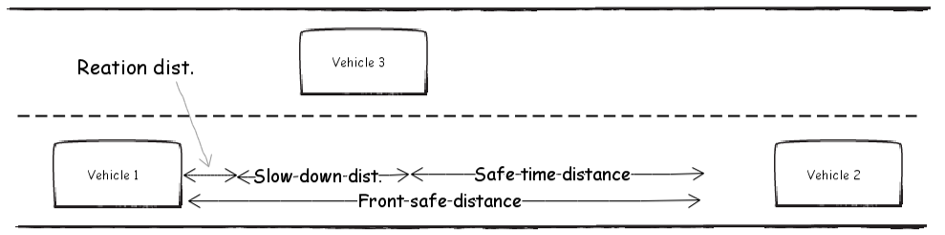
\includegraphics[width=0.90\textwidth,height=0.90\textheight,keepaspectratio]{figures/Chapter_4/4_front_safe_distance.png}
\centering
\protect\caption{\label{fig:4_2_3_3-1}\textit{Front safe distance} of \textit{\mbox{Vehicle 1}} to the closest front \textit{\mbox{Vehicle 2}}}
\end{figure}

For example with \textit{\mbox{Vehicle 1}} \mbox{speed  = 30 m/s},  \textit{\mbox{Vehicle 2}} \mbox{speed = 28 m/s}, braking acceleration = \mbox{4 m/$s^2$} and simulator iteration \mbox{time = 0.1} s then \textit{Front safe distance} of \textit{\mbox{Vehicle 1}}  is \mbox{77.5 m}. If the distance between \textit{\mbox{Vehicle 1}} and \textit{\mbox{Vehicle 2}} is smaller \textit{\mbox{Vehicle 1}} has to react on this situation.

If the front \textit{\mbox{Vehicle 2}} is faster at least 1 m/s (ex. 31m/s) than back \textit{\mbox{Vehicle 1}}, \textit{Slow down distance} will be equal 0, as we mentioned before. Because the \textit{\mbox{Vehicle 2}}  is faster than \textit{\mbox{Vehicle 1}} the \textit{Safe time distance} is decreased to 80\% to avoid pointless actions (slowing down \textit{\mbox{Vehicle 1}}, the real distance between \textit{\mbox{Vehicle 1}} and \textit{\mbox{Vehicle 2}}   is less than \textit{Front safe distance}; more about the behaviour rule in part Vehicle behaviour in this section).  \textit{Safe time distance} could be reduced, because then \textit{\mbox{Vehicle 2}} is faster and therefore real \textit{Front safe distance} will be increasing in time and probability of crash is minimal.

According to observation of real traffic we added an exception for case that the front \textit{\mbox{Vehicle 2}} is truck, then the \textit{Safe time distance} is reduced to 40\% of normal distance, because truck braking path is longer than that of the car.

\paragraph{\textit{Overtaking distance}}

is distance that the overtaking vehicle (\textit{\mbox{Vehicle 1}}, Figure \ref{fig:4_2_3_3-2}) must be in front of the overtaken vehicle (\textit{\mbox{Vehicle 2}}) to be able to safely change into the lane (\textit{\mbox{Vehicle 2}} lane). This distance defines, how far the vehicle should be to overtake the back vehicle in dependency of their speed difference.

\begin{figure}[ph]
\centering
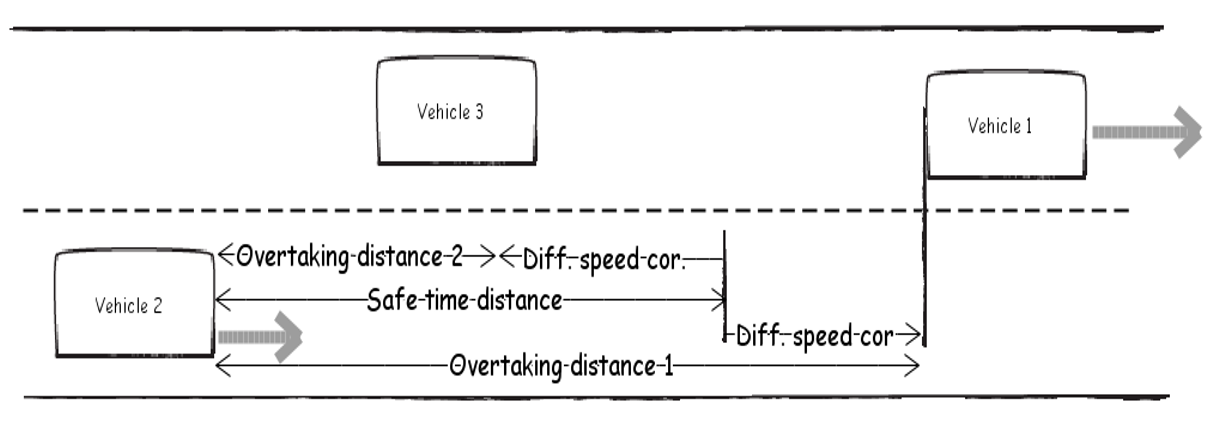
\includegraphics[width=0.90\textwidth,height=0.90\textheight,keepaspectratio]{figures/Chapter_4/4_overtaking_distance.png}
\centering
\protect\caption{\label{fig:4_2_3_3-2}\textit{Overtaking distance} of \textit{\mbox{Vehicle 1}} to closest back vehicle in lower lane \textit{\mbox{Vehicle 2}}}
\end{figure}

As you can see in Figure \ref{fig:4_2_3_3-2}, \textit{Overtaking distance} of \textit{\mbox{Vehicle 1}} at destined lane (in that figure it is in the right lane) consists of \textit{Safe time distance} of the closest back \textit{\mbox{Vehicle 2}} in the lane and Difference speed correction. \textit{Different speed correction} is added to the \textit{Safe time distance} if \textit{\mbox{Vehicle 1}} is slower than \textit{\mbox{Vehicle 2}}. Otherwise the \textit{Safe time distance} is decreased by the \textit{Different speed correction}. 

So in Figure \ref{fig:4_2_3_3-2}, \textit{Overtaking distance} of \textit{\mbox{Vehicle 1}} from \textit{\mbox{Vehicle 2}} is \textit{Overtaking distance} 1, if \textit{\mbox{Vehicle 1}} is faster than the closest back \textit{\mbox{Vehicle 2}}. Whether \textit{\mbox{Vehicle 1}} would be slower than \textit{\mbox{Vehicle 2}}, the \textit{Overtaking distance} of \textit{\mbox{Vehicle 1}} in right lane from \textit{\mbox{Vehicle 2}} would be \textit{Overtaking distance} 2. This situation appears in case of unusual \textit{\mbox{Vehicle 1}} driver’s behaviour in overtaking movement, when he does not respect safety rules.

\paragraph{Changing of lane}

- Every vehicle can change lane, but it cannot endanger itself and the others by this action, so there has to be free safety space. The vehicle changing lane can move in space between two other vehicles in the target lane only if next two conditions are met.

\begin{enumerate}
\item The space in front of the changing vehicle in target lane must be bigger than its \textit{Front safe distance}.
\item There has to be free back space to the vehicle in the lane which is bigger as \textit{Overtaking distance} of the changing vehicle.
\end{enumerate}

You can see the conditions in the following Figure \ref{fig:4_2_3_3-3}. In this figure you can see main \textit{\mbox{Vehicle 1}} in \textit{lane 1} with the conditions for changing of lane. You can see that \textit{\mbox{Vehicle 1}} cannot turn to \textit{lane 2}, although its \textit{Front safe distance} is smaller than the distance to the closest front \textit{\mbox{Vehicle 5}} in the \textit{lane 2}  but  \textit{\mbox{Vehicle 1}} \textit{Overtaking distance} is smaller than the distance to \textit{\mbox{Vehicle 4}}. On the other side \textit{\mbox{Vehicle 1}} can turn to \textit{lane 0} because its \textit{Overtaking distance} and \textit{Front safe distance} are smaller than both distances to the closest back \textit{\mbox{Vehicle 2}} and front \textit{\mbox{Vehicle 3}} in \textit{lane 0}.

\begin{figure}[ph]
\centering
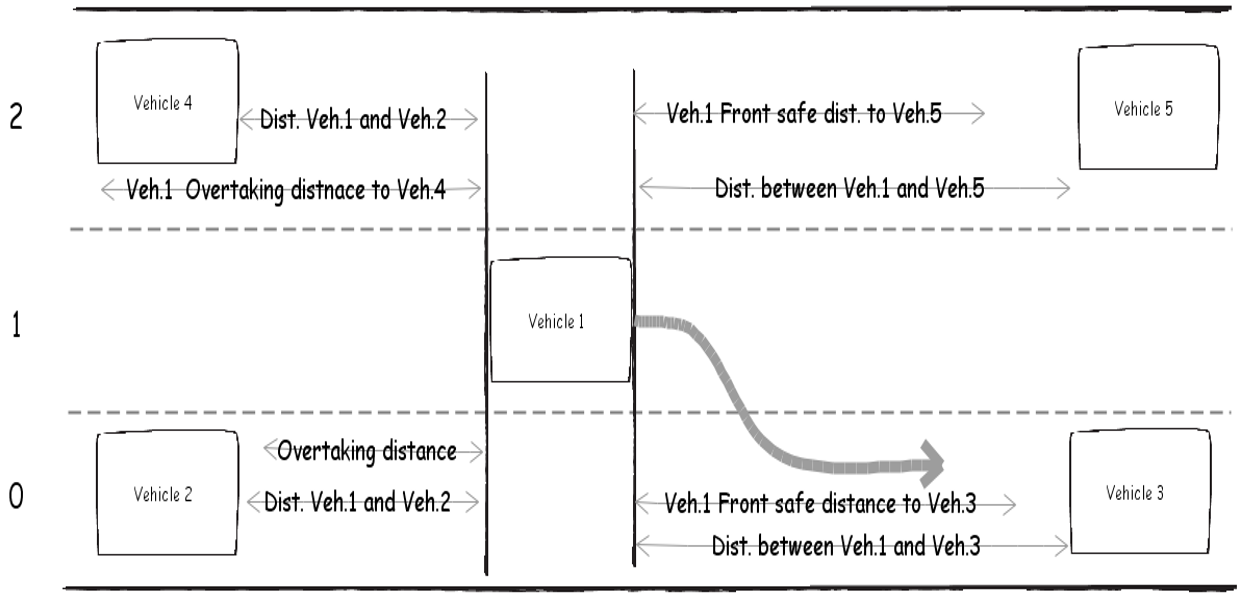
\includegraphics[width=0.90\textwidth,height=0.90\textheight,keepaspectratio]{figures/Chapter_4/4_changing_lanes.png}
\centering
\protect\caption{\label{fig:4_2_3_3-3}Possibilities of \textit{\mbox{Vehicle 1}} to change lane and vehicles which can influence the it}
\end{figure}

During the changing of lane, \textit{Preferred speed} of changing vehicle is modified too. If a vehicle turns to left lane, to the faster one, its speed is increased by 1 m/s. For turning to right lane, to slower one, its speed is decreased by the same value.

\paragraph{Behaviour of vehicles}

- According to the situation on the highway, regular vehicle which is not part of a platoon has 4 options to do, as you can see in decision tree in Figure \ref{fig:4_2_3_3-4} :

\begin{itemize}
\item Speed up, but maximally to its \textit{Preferred speed} and stay in the lane, 
\item Slow down and stay in the lane,
\item Turn to the left lane and speed up, 
\item Turn to the right lane. 
\item Continue without any actions. 
\end{itemize}

\begin{figure}[ph]
\centering
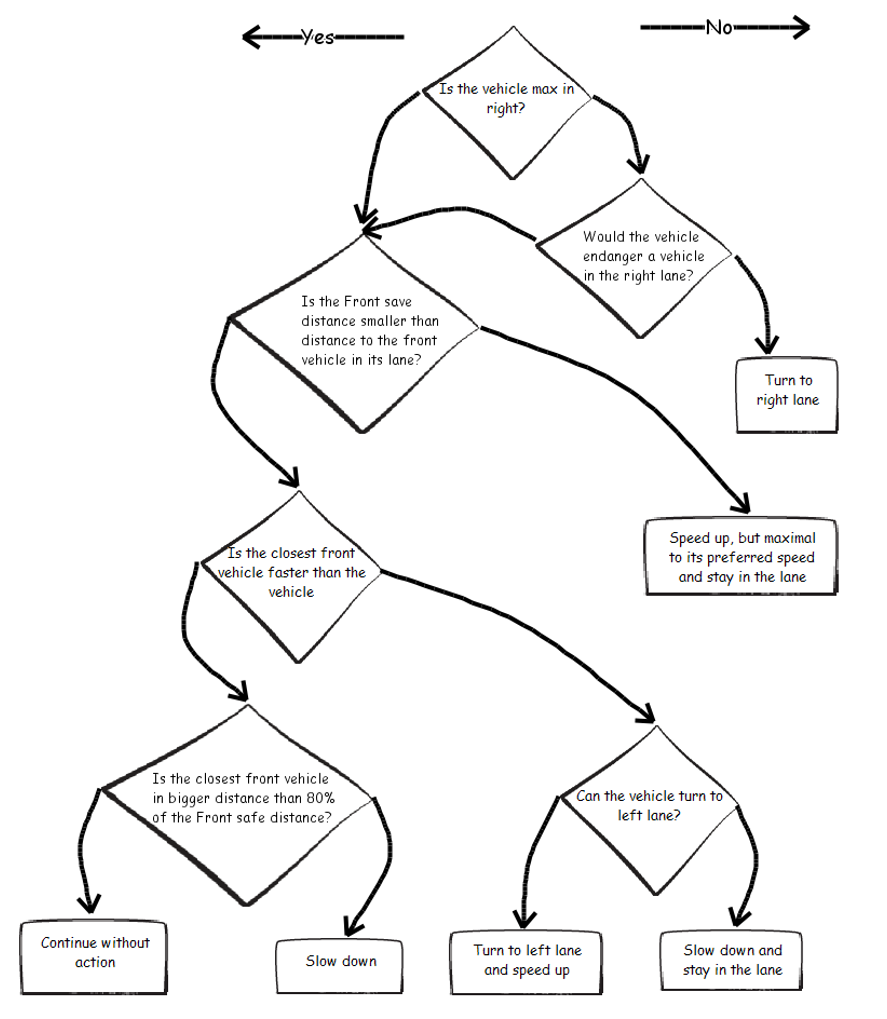
\includegraphics[width=0.95\textwidth,height=0.95\textheight,keepaspectratio]{figures/Chapter_4/4_diagram.png}
\centering
\protect\caption{\label{fig:4_2_3_3-4}Decision diagram of behaviour of passenger vehicle agent in simulator}
\end{figure}

The first rule which every vehicle should observe is to drive on the right side according to Czech law. So if the situation allows it, every vehicle turns to right lane and travels there. This movement is called Changing to slower lane and you can see it in Figure \ref{fig:4_2_3_3-5}. In this example you can see that \textit{\mbox{Vehicle 1}} can according to rule Changing of lane turn to right lane.

\begin{figure}[ph]
\centering
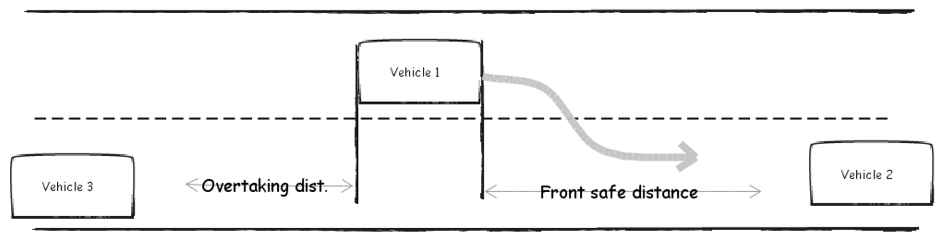
\includegraphics[width=0.90\textwidth,height=0.90\textheight,keepaspectratio]{figures/Chapter_4/4_changing_slower_lane.png}
\centering
\protect\caption{\label{fig:4_2_3_3-5}Situation when \textit{\mbox{Vehicle 1}} can turn to slower lane between \textit{\mbox{Vehicle 2}} and \textit{\mbox{Vehicle 3}}}
\end{figure}

The second rule is to keep preferred speed by overtaking.  As we mentioned before, every vehicle has its \textit{Preferred speed} and tries to stay at this speed level most of the time, so if it can increase its speed to this level, it does it so and this is the second main rule for behaviour of every vehicle. In order to achieve this speed level the vehicle changes its lane to the faster one to avoid its deceleration by some vehicle which goes in front of it in the same lane. This action is called overtaking see in Figure \ref{fig:4_2_3_3-6}. In this example let’s assume that \textit{Vehicles 1}  speed is higher than \textit{\mbox{Vehicle 2}} speed. The distance between these two vehicles in time becomes smaller than the \textit{Front safe distance} of \textit{\mbox{Vehicle 1}} to \textit{\mbox{Vehicle 2}},  then \textit{\mbox{Vehicle 1}} should decide. It prefers overtaking to decelerating and therefore \textit{\mbox{Vehicle 1}} does the overtaking movement to the left lane, respecting Changing of lane condition.

\begin{figure}[ph]
\centering
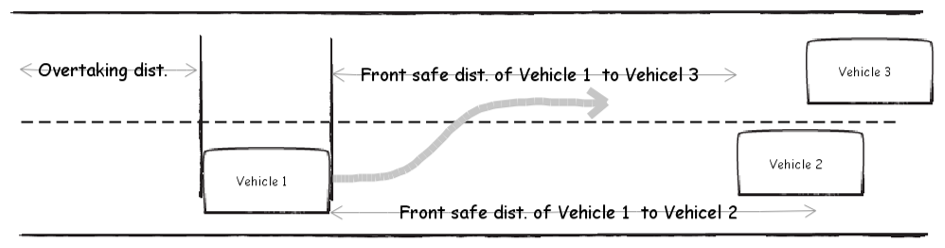
\includegraphics[width=0.90\textwidth,height=0.90\textheight,keepaspectratio]{figures/Chapter_4/4_can_overtake.png}
\centering
\protect\caption{\label{fig:4_2_3_3-6}Situation when \textit{\mbox{Vehicle 1}} can overtake Vehicle\-2 and turn to faster lane behind \textit{\mbox{Vehicle 3}}}
\end{figure}

The next rule is to drive safely by keeping \textit{Front safe distance}. If in front of the vehicle, let us call it \textit{\mbox{Vehicle 1}}, there is another vehicle, \textit{\mbox{Vehicle 2}}, whose speed is smaller than that of \textit{\mbox{Vehicle 1}} and that \textit{\mbox{Vehicle 1}} cannot overtake, \textit{\mbox{Vehicle 1}} has to decrease its speed according to the safe distance in the lane. Like example in Figure \ref{fig:4_2_3_3-7}, which is very similar to previous example, instead of that, the distance between \textit{\mbox{Vehicle 1}} and \textit{\mbox{Vehicle 3}} is smaller than the \textit{Front safe distance} of \textit{\mbox{Vehicle 1}} to \textit{\mbox{Vehicle 3}}. So according to safety rule of Changing of lane, \textit{\mbox{Vehicle 1}} cannot overtake and has to slow down.

\begin{figure}[ph]
\centering
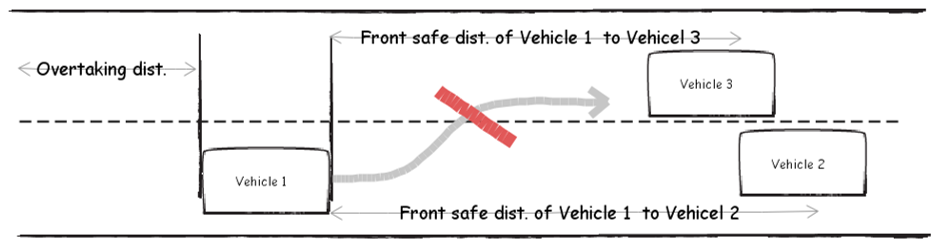
\includegraphics[width=0.90\textwidth,height=0.90\textheight,keepaspectratio]{figures/Chapter_4/4_cannot_overtake.png}
\centering
\protect\caption{\label{fig:4_2_3_3-7}Situation when \textit{\mbox{Vehicle 1}} cannot overtake \textit{\mbox{Vehicle 2}} and turn to faster lane behind \textit{\mbox{Vehicle 3}}}
\end{figure}

\subsection{Platooning}

The PlatooningCentreModule, as the name refers, is responsible for platooning concept. Similarly as it is in VehicleGenerationModule, platoons are also generated in every lane (according to vehicle type) and only at beginning of simulation. They are not created during simulation from single vehicles if the vehicles sequence is changed because of overtaking and changing lanes. And it is not allowed to add vehicle into platoon during simulation. But the platoons could decomposite because of other vehicle drivers' behaviour.

It is not allowed to create a platoon from vehicles, which are already in another one. The number of following vehicles in platoon is generated from VehicleGenerationModule data according to a uniform distribution in interval from 0 to set parameter.

In this thesis we do not deal with internal control system between vehicles in platoon, such as keeping constant distance and speed between vehicles, turning of vehicles, behaviour features, etc. For this work we assume full-functioning platooning model and we test higher highway traffic principles and platoons are part of this traffic as one “entity”. 

Platoons are implemented by one main lead vehicle and many following vehicles. The lead vehicle is responsible for platoon behaviour and influences behaviour of all following vehicles in platoon. It decides about platoon behaviour and sends platoon orders to the rest of the vehicles in platoon. They fulfil this platoon orders of their lead vehicles. Every order contains what the vehicle should do and the location where the order should be filled. The following vehicles independently keep nearly constant distance from the lead vehicle, they speed up or down a little if the distance is bigger or smaller than the required one.

There are implemented three types of changing of lane by platoon:

\begin{itemize}
\item Snake

If the lead vehicle finds out, that it will overtake, it sends platoon order to change lane in the fix location, it means in the same location as the lead vehicle did, in location that lead vehicle decided to change lane, to overtake front vehicle. It is displayed in Figure \ref{fig:4_2_3_3-8}. You can see that this action depends only on \textit{Front safe distance} in the lane and \textit{Overtaking distance} of lead vehicle \textit{\mbox{Vehicle 1}}.

\begin{figure}[ph]
\centering
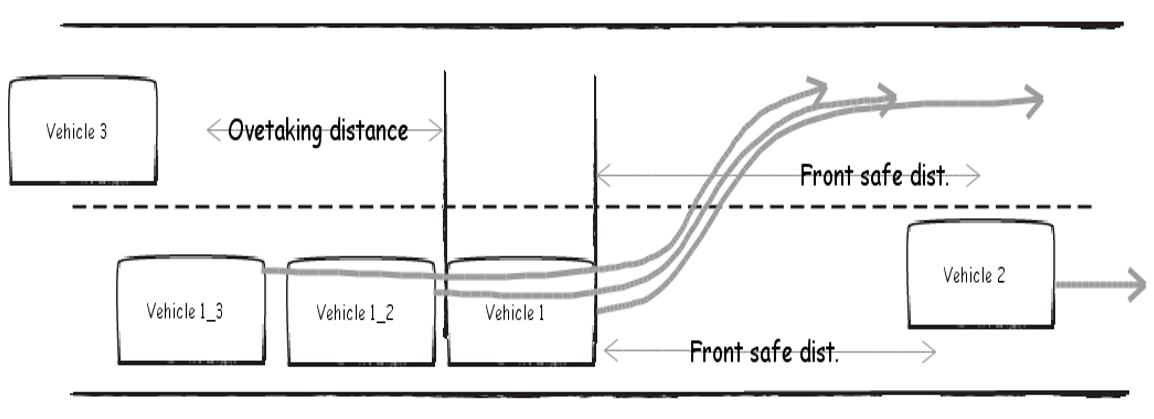
\includegraphics[width=0.90\textwidth,height=0.90\textheight,keepaspectratio]{figures/Chapter_4/4_overtaking_snake.png}
\centering
\protect\caption{\label{fig:4_2_3_3-8}Platoon overtaking type: Snake}
\end{figure}

\item All at once

It is more cooperative approach, all (leading and following) vehicles change a lane at the same time. A platoon starts overtaking action, if there is no vehicle in space defined by position of last platoon vehicle minus its \textit{Overtaking distance} and position of lead vehicle plus its \textit{Front safe distance}. See Figure \ref{fig:4_2_3_3-9}.

\begin{figure}[ph]
\centering
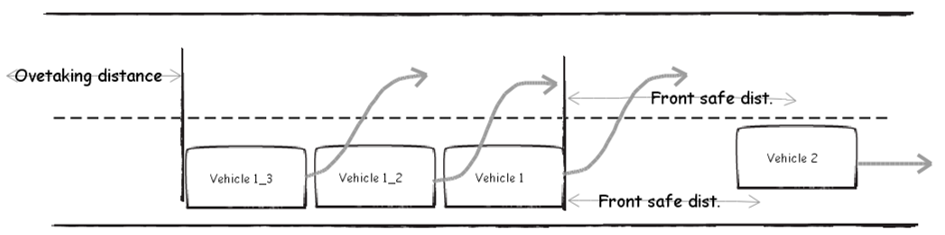
\includegraphics[width=0.90\textwidth,height=0.90\textheight,keepaspectratio]{figures/Chapter_4/4_overtaking_allatonce.png}
\centering
\protect\caption{\label{fig:4_2_3_3-9}Platoon overtaking type: All at once}
\end{figure}

\item Last first - All at once with preparation

If the platoon cannot change lane by All at once , the Change of lane movement is realized in two steps, as you can see in Figure \ref{fig:4_2_3_3-10}. The first step is change of lane only by the last platoon \textit{\mbox{Vehicle 1 3}} to get free space in the lane for rest of the platoon vehicles, potentially to slow down \textit{\mbox{Vehicle 4}} if it is fast one but far. In the figure you can see, that in this step \textit{\mbox{\mbox{Vehicle 1}}} cannot do overtaking movement because of \textit{\mbox{Vehicle 3}}. 

But \textit{\mbox{Vehicle 3}} drives faster than the platoon of \textit{\textit{\mbox{\mbox{Vehicle 1}}}} and step two is realised in some seconds later as you can see in Figure \ref{fig:4_2_3_3-11}, and where also the rest of platoon vehicles can do overtaking movement.

\begin{figure}[ph]
\centering
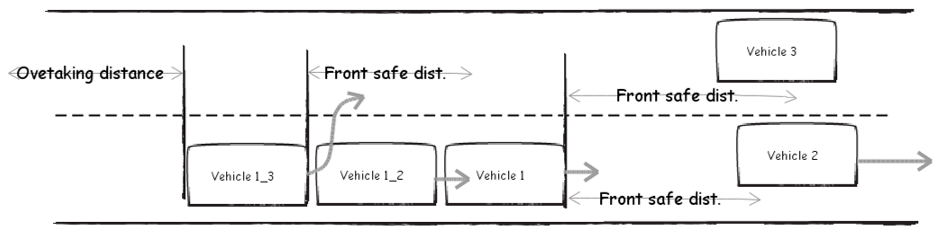
\includegraphics[width=0.90\textwidth,height=0.90\textheight,keepaspectratio]{figures/Chapter_4/4_overtaking_lastFirst1.png}
\centering
\protect\caption{\label{fig:4_2_3_3-10}Platoon overtaking type: Last First - step 1}
\end{figure}


\begin{figure}[ph]
\centering
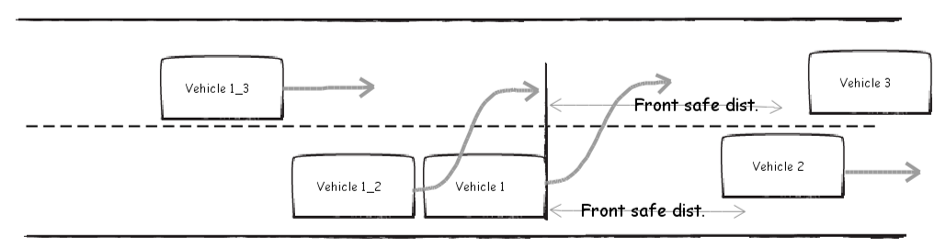
\includegraphics[width=0.90\textwidth,height=0.90\textheight,keepaspectratio]{figures/Chapter_4/4_overtaking_lastFirst2.png}
\centering
\protect\caption{\label{fig:4_2_3_3-11}Platoon overtaking type: Last first - step 2}
\end{figure}


\end{itemize}

\subsubsection*{Collisions during overtaking}

Snake type of overtaking depends only on the Lead vehicle of the platoon and does not depend on location of rest following vehicles in the platoon. In real situation , if  some following vehicle in the  platoon gets to close to another vehicle, this following  vehicle has to leave the platoon and becomes Lead vehicle of a new platoon- see Figure \ref{fig:4_2_3_3-12}.

\begin{figure}[ph]
\centering
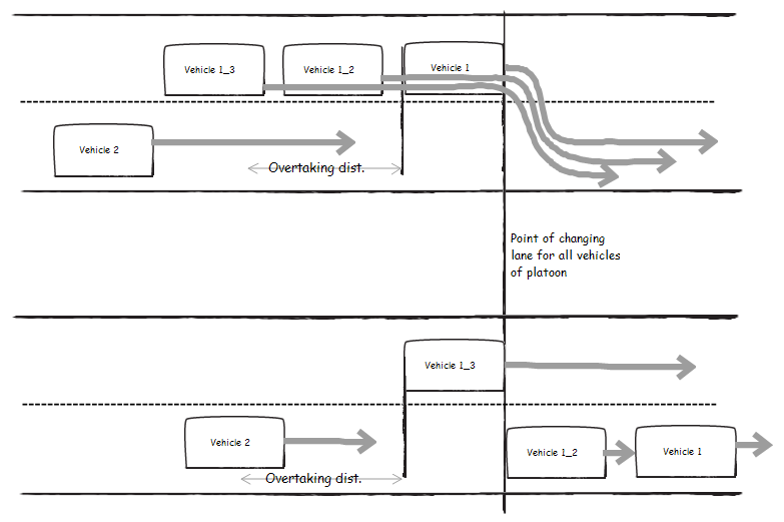
\includegraphics[width=0.90\textwidth,height=0.90\textheight,keepaspectratio]{figures/Chapter_4/4_platoon_decomposition.png}
\centering
\protect\caption{\label{fig:4_2_3_3-12}Conditions and process of decomposition of a platoon}
\end{figure}







\section[Main features of traffic situation measured during the simulation]{Main features of traffic situation measured \newline during the \mbox{simulation}\sectionmark{Main features of traffic...}}
\sectionmark{Main features of traffic...}

There are many features which can be studied. We decided to focused on some, which seemed important to us. There is a list of features, which are predefined in the simulator to be measured.

\begin{itemize}
\item Density of traffic – is the number of vehicles that pass a defined highway in a point per time period without breaking any safety rules that are set in our simulator. This point is at the beginning of simulated part of highway, because the agents (vehicles, platoons) are added only in this point. It is counted as ration of number of all generated vehicles and total time of simulation. To achieve maximum capacity it is necessary to set \textit{Generation limit} to false (parameter is mentioned in Section 4.2.2).
\item Average speed of all vehicles 
\item Average speed of all passenger vehicles
\item Total speed dispersion
\item Average speed of vehicles in each lane
\item Speed dispersion in each lane
\item Actual number of placed vehicles in highway – it is number of vehicles that are “going” in highway at that moment, at the time
\item Actual number of placed vehicles in each lane
\item Frequency of collisions – number of collisions per hour in simulated environment; collision is a situation, if the distance between the vehicle and the  closest front vehicle in less than 60\% of its \textit{Front safe distance} 
\end{itemize}

 

\chapter[Experiments of platooning concept in traffic simulator]{Experiments of platooning concept in traffic simulator\chaptermark{Experiments of platooning concept}}
\chaptermark{Experiments of platooning concept}

This chapter covers testing of platooning concept in our developed traffic simulator (see Chapter 4). By parameters which are mentioned in Section 4.2.2 and by the selection of the highway type we simulated and checked positive effects of platooning concept on highway traffic. Later in this chapter there are descriptions and commentaries of several tests and simulations that correspond to the maximum and real utilisation of highway. We simulated 3 types of highway – one, two and three-lane highway – and length of highway segments is 5 km.

The main feature of traffic which we studied and compared was maximum capacity of highway and average speed of passenger vehicles. Because of long duration (12 minutes) of tests, we were not able to do more than two times and do statistical calculations of these features. Instead of that we used a value at which the capacity of simulator stabilized as maximum capacity and average speed of passenger vehicles during last 10 minutes of test (2 minutes to fill the simulation environment).








\section[Experiment \#1: Maximum capacity of lane in simulator]{Experiment \#1: Maximum capacity of lane in simulator\sectionmark{Experiment \#1...}}
\sectionmark{Experiment \#1...}

In this experiment we tried to find out maximum capacity of one highway lane in our simulator with different ratio between platooning and non-platooning passenger vehicles. Because we used very similar preconditions, we expected very similar results to the theoretical example which is described in Section 2.5. In order to confirm this assumption we compared results only for percentage of platooning vehicles equal to 0\% and 100\%, because the Equation \ref{eq:max_cap_platooning} is not defined for more values.





\subsection*{Simulator setting for the test}
\begin{itemize}
\item Average speed: 25 m/s, 30 m/s, 35 m/s
\item Speed dispersion: 0 m/s
\item Length of platoon: 6
\item Number of lanes:  1
\item Platooning vehicles ratio: 0\%, 20\%, 40\%, 60\%, 80\%, 100\%
\item Generation limit: false
\item Generate trucks: false
\end{itemize}



\subsection*{Experiment result}

In Figure \ref{fig:5_1-1} and Table \ref{tab:5_1-1} you can see dependency of maximum capacity of lane and percentages of platooning vehicles. The maximum capacity is a nonlinear dependence on percentage of platooning vehicles. 

\begin{figure}[ph]
\centering
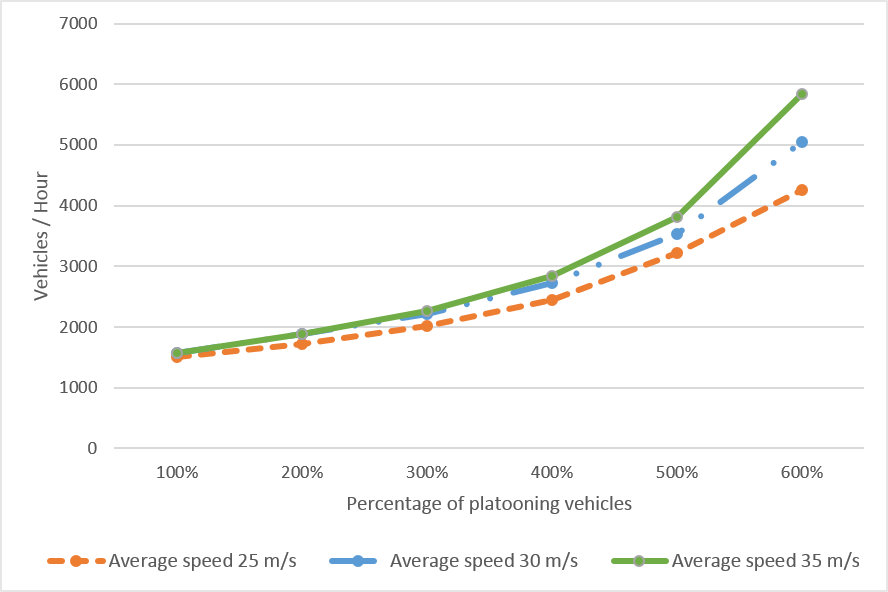
\includegraphics[width=0.82\textwidth,height=0.82\textheight,keepaspectratio]{figures/Chapter_5/5_maximum_cap.png}
\centering
\protect\caption[Maximum capacity of one lane for 25 m/s, 30 m/s, 35 m/s]{\label{fig:5_1-1}Maximum capacity of one lane for 25 m/s, 30 m/s, 35 m/s - capacity measured only for 0\%, 20\%, 40\%, 60\%, 80\%, 100\% platooning vehicles, so as to be more visual the line connecting measured data was added}
\end{figure}

\begin{table}[ph]
\begin{centering}
\begin{tabular}{|c|c|c|c|c|c|c|}
\hline 
Average speed / Platooning \% &	0\% &	20\% &	40\% &	60\% &	80\% &	100\%\tabularnewline
\hline 
25 m/s &	1 575 &	1 839 &	2 190 &	2 725 &	3 513 &	5 015\tabularnewline
\hline 
30 m/s &	1 504 &	1 760 &	2 116 &	2 701 &	3 528 &	5 408\tabularnewline
\hline 
35 m/s &	1 566 &	1 852  & 2 224 &	2 825 &	3 814 &	5 832\tabularnewline
\hline 
\end{tabular}
\centering
\protect\caption{\label{tab:5_1-1}Measured values of maximum capacity of lane for different average speed}
\end{centering}
\end{table}

We expected that our maximum capacity of lane results from simulator should have been similar to calculated values which we got by solving Equation \ref{eq:max_cap_platooning}. In Tables \ref{tab:5_1-2}, \ref{tab:5_1-3} there are comparisons of the calculated Theoretical maximum capacity of lane and of our adequate reached values from Table \ref{tab:5_1-1}. 

\begin{table}[ht]
\begin{centering}
\begin{tabular}{|c|c|c|c|}
\hline 
Experiment / & 	Simulator 0\%  & 	Theoretical 0\%   &	Ratio  \tabularnewline
 Maximum lane & 	 platooning & 	  platooning  &	 (Reached / \tabularnewline
 capacity& 	  vehicles & vehicles & Theoretical)\tabularnewline
\hline 
Average speed 25 m/s &	1 575 &	1 666 &	94.54\%\tabularnewline
\hline 
Average speed 30 m/s &	1 524 &	1 688 &	90.31\%\tabularnewline
\hline 
Average speed 35 m/s &	1 566 &	1 702 &	92.01\%\tabularnewline
\hline 
\end{tabular}
\centering
\protect\caption{\label{tab:5_1-2}Comparison of maximum reached value and maximum theoretical values of maximum lane capacity for 0\% platooning vehicles}
\end{centering}
\end{table}

\begin{table}[ht]
\begin{centering}
\begin{tabular}{|c|c|c|c|}
\hline 
Experiment /  & Simulator 100\% & 	Theoretical 100\%   &	Ratio \tabularnewline
 Maximum lane &  platooning  & 	 platooning  &	 (Reached / \tabularnewline
 capacity& vehicles & 	 vehicles &	 Theoretical)\tabularnewline
\hline 
Average speed 25 m/s & 5 015 &	5 129 &	97.78\%\tabularnewline
\hline 
Average speed 30 m/s & 	5 408 &	5 684 &	95.14\%\tabularnewline
\hline 
Average speed 35 m/s&	5 842 &	6 097 &	95.82\%\tabularnewline
\hline 
\end{tabular}
\centering
\protect\caption{\label{tab:5_1-3}Comparison of maximum reached value and maximum theoretical values of maximum lane capacity for 100\% platooning vehicles}
\end{centering}
\end{table}

All our reached values for 0\% platooning vehicles are up to 10\% less than the theoretical ones. It is caused by our different approach to safe distance which should be in front of the vehicle. In our case the Front safe distance to vehicle of the same speed consists of \textit{Reaction distance} and \textit{Safe time distance}. The example does not count with the \textit{Reaction distance}. It is also influenced by changing speed of vehicles which oscillate around optimal distance to a front vehicle. The reached values for 100\% platooning have smaller percentage mistake up to 5\%, because the \textit{Reaction distance} is contained in Front safe distance, which effects only the leading vehicles of each platoon. 

We think that this less than 10\% difference proves that the simulator can be used for testing of maximum capacity of highway with platooning concept.

For other next experiments we used simulation with an average speed, zero speed dispersion, constant platooning length, no generation limit and no trucks as a reference value for maximum capacity of a lane and the average speed over different percentage of platooning vehicles.

















\newpage

\section[Experiment \#2: Linear dependency of maximum highway capacity on number of its lanes]{Experiment \#2: Linear dependency of maximum highway capacity on number of its lanes\sectionmark{Experiment \#2...}}
\sectionmark{Experiment \#2...}

We wanted to verify whether the maximum capacity is proportional to number of lanes with overtaking. We expected the proportionality, because number of overtaking and changing lanes actions will be very low thanks to \textit{Speed dispersion} = 0. We tried to prove it by comparison of multiplies of one-lane highway capacity with two-lane highway capacity and three-lane highway capacity.







\subsection*{Simulator setting for the test}
\begin{itemize}
\item Average speed: 30 m/s
\item Speed dispersion: 0 m/s
\item Length of platoon: 6
\item Number of lanes:  1, 2, 3
\item Platooning vehicles ratio: 0\%, 20\%, 40\%, 60\%, 80\%, 100\%
\item Generation limit: false
\item Generate trucks: false
\end{itemize}



\subsection*{Experiment result}

In Table \ref{tab:5_2-1} there are results of maximum capacity of highway with different numbers of lanes and with different percentage of platooning vehicles. All generated vehicles had the same speed. In the next Table \ref{tab:5_2-2} there is percentage comparison of maximum capacity of two-lane and three-lane highway with adequate multiple of maximum capacity of one-lane highway. Since the maximum capacity of multi-lane highways is almost always smaller than multiplies of the one-lane highway, the maximum capacity of highway in our simulator is not exactly proportioned to the number of lanes, but it is very close to it.

\begin{table}[ht]
\begin{centering}
\begin{tabular}{|c|c|c|c|c|c|c|}
\hline 
Type / Platooning \% &	0\% &	20\% &	40\% &	60\% &	80\% &	100\%\tabularnewline
\hline 
1 lane highway &	1 504 &	1 760 &	2 116 &	2 701 &	3 528 &	5 408\tabularnewline
\hline 
2 lane highway &	3 015 &	3 552 &	4 214 &	5 218 &	7 016 &	10 290\tabularnewline
\hline 
3 lane highway &	4 462 &	5 186 &	6 250 &	7 748 &	10 285 &	15 034\tabularnewline
\hline 
\end{tabular}
\centering
\protect\caption{\label{tab:5_2-1}Measured maximum capacity of highway with 1, 2 and 3 lanes for percentage of platooning vehicles}
\end{centering}
\end{table}

\begin{table}[ht]
\begin{centering}
\begin{tabular}{|c|c|c|c|c|c|c|}
\hline 
Ratio / Platooning \% &	0\% &	20\% &	40\% &	60\% &	80\% &	100\%\tabularnewline
\hline 
2 lane highway &	1.0017 &	1.0090 &	0.9956 &	0.9658 &	0.9942 &	0.9514\tabularnewline
/ triple of 1 lane highway & & & & & &\tabularnewline
\hline 
3 lane highway &	0.9883 &	0.9821 &	0.9844 &	0.9560 &	0.9716 &	0.9267\tabularnewline
/ triple of 1 lane highway & & & & & &\tabularnewline
\hline 
\end{tabular}
\centering
\protect\caption{\label{tab:5_2-2}Ratio of multi-lanes highways maximum capacities and adequate multiple of maximum capacity of one lane highway}
\end{centering}
\end{table}



















\section[Experiment \#3: Maximum capacity of two lane highway with real traffic conditions of Czech Republic]{Experiment \#3: Maximum capacity of two lane highway with real traffic conditions of Czech Republic\sectionmark{Experiment \#3...}}
\sectionmark{Experiment \#3...}


In real situation all vehicles would never travel by  the same speed level. So this experiment is focused on effects of platooning concept in Czech highway environment with the speed based on research which is mentioned in Chapter 2. We set main parameters of our simulator (Chapter 4) and we run the simulation of highway of length 5 km for 15 minutes to find out, how the traffic would behave for different percentage of platooning vehicles. 

We expected positive effect on maximum capacity of highway and negative effect on average speed of passenger vehicles, because long platoon of slower vehicles should more slow down the lane and because the overtaking vehicles have to overtake long platoons for longer time too. 






\subsection*{Simulator setting for the test}

\begin{itemize}
\item Average speed: 34 m/s
\item Speed dispersion: 3 m/s
\item Length of platoon: 2-6
\item Number of lanes:  2
\item Platooning vehicles ratio: 0\%, 20\%, 40\%, 60\%, 80\%, 100\%
\item Generation limit: false
\item Generate trucks: false, true
\item Percentage of passenger vehicles in traffic: 65\%
\item Overtaking: Snake type
\end{itemize}

\subsection*{Experiment results}

We did simulations with traffic in two-lane highway without truck traffic (see maximum reached capacity during time in Figure \ref{fig:5_3-1}) and with included truck traffic (See level of maximum reached capacity during time in Figure \ref{fig:5_3-2}).

\begin{figure}[ph]
\centering
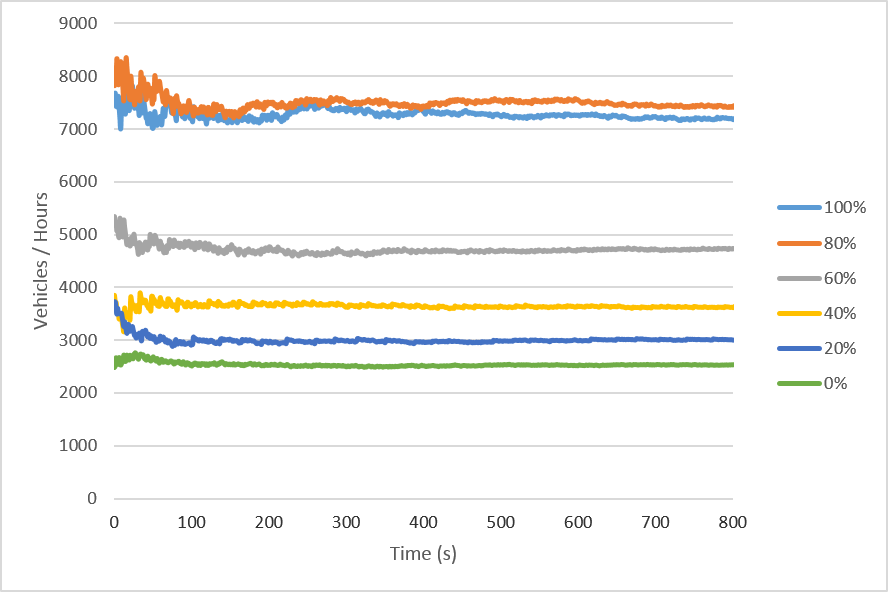
\includegraphics[width=0.82\textwidth,height=0.82\textheight,keepaspectratio]{figures/Chapter_5/5_max_2lane_Ntrucks.png}
\centering
\protect\caption[Maximum capacity of two-lane highway and real traffic conditions without trucks]{\label{fig:5_3-1}Maximum capacity of two-lane highway and real traffic conditions without trucks}
\end{figure}



\begin{figure}[ph]
\centering
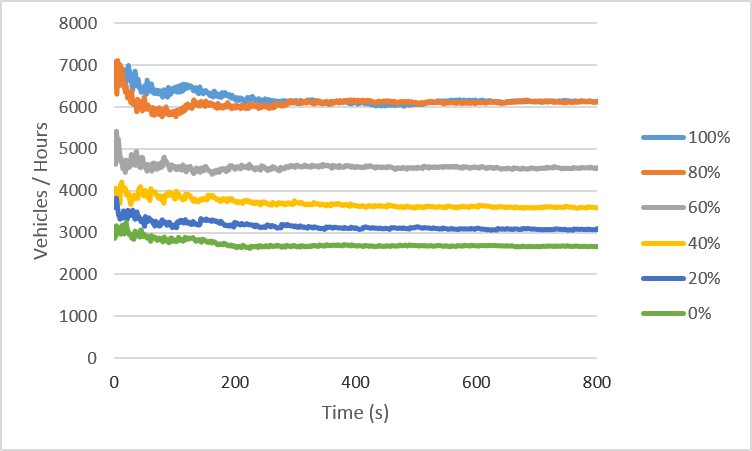
\includegraphics[width=0.82\textwidth,height=0.82\textheight,keepaspectratio]{figures/Chapter_5/5_max_2lane_trucks.png}
\centering
\protect\caption[Maximum capacity of two-lane highway and real conditions with trucks]{\label{fig:5_3-2}Maximum capacity of two-lane highway and real conditions with trucks}
\end{figure}



As we expected, in Figure \ref{fig:5_3-4} we can see positive effect of platooning concept on maximum capacity of two-lane highway with realistic conditions. 

This confirmed our assumption that there is some relation between percentage of platooning vehicles and the average speed during maximum usage of highway. There is a tendency that the average speed is decreasing with increasing percentage of platooning vehicles, this can be seen in Figure \ref{fig:5_3-3}.

\begin{figure}[ph]
\centering
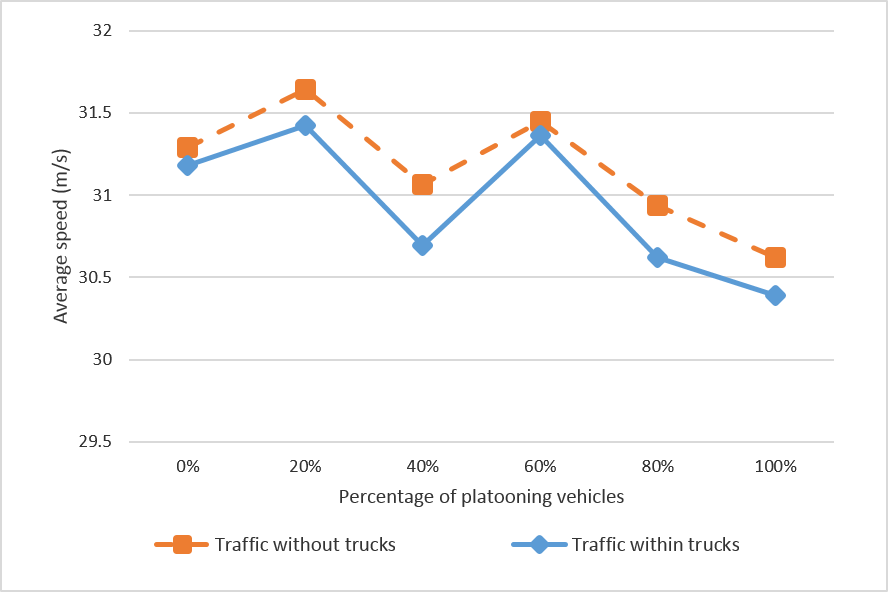
\includegraphics[width=0.82\textwidth,height=0.82\textheight,keepaspectratio]{figures/Chapter_5/5_E3_avgSpeed.png}
\centering
\protect\caption[Average speed of traffic without and with trucks in two-lane highway]{\label{fig:5_3-3}Average speed of traffic without and with trucks in two-lane highway  - average speed measured after stabilization of traffic and only for 0\%, 20\%, 40\%, 60\%, 80\%, 100\% platooning vehicles, so as to be more visual the line connecting measured data was added.}
\end{figure}

As it can be seen in both tests, maximum capacity (Figure \ref{fig:5_3-1} and Figure \ref{fig:5_3-2}) and average speed were generally higher in the start of simulation, but during time, after the full filling of highway, they have stabilized at lower levels. So we took maximum capacity of each simulation at the end of the simulation and put them into Table \ref{tab:5_3-1}. In this table you can also see the percentage ration of our reached maximum capacity and double of theoretical maximum lane capacity which we got by the same way as in Experiment \#1 but for average speed 34 m/s. Results can be seen also in Figure \ref{fig:5_3-4}.

We repeated the test several times and the results were always same. It is interesting that in real traffic conditions there is not a big difference between maximum capacity of highway for 80\% and 100\% platooning vehicles. We did not find the reason of that.

\begin{table}[ph]
\begin{centering}
\begin{tabular}{|c|c|c|c|c|c|c|}
\hline 
... / Platooning \%&	0\% &	20\% &	40\% &	60\% &	80\% &	100\%\tabularnewline
\hline 
Theoretical maximum &	3 150 &	3 862 &	4 560 &	5 748 &	7 756 &	11 622\tabularnewline
 capacity for 2 lane highway & & & & & &\tabularnewline
\hline 
Reached maximum capacity & 2 528 &	2 986 &	3 629 &	4 693 &	7 290 &	7 262\tabularnewline
for traffic without trucks & & & & & &\tabularnewline
\hline 
Ratio Theoretical maximum & & & & & &\tabularnewline
capacity / Reached maximum & 80.27\% &	77.32\%	 & 79.58\% &	81.65\% &	93.99\% &	62.48\%
\tabularnewline
capacity without trucks & & & & & &\tabularnewline
\hline 
Reached maximum capacity & 2 664 &	3 059 &	3 617 &	4 490 &	6 144 &	6 163\tabularnewline
for traffic with trucks & & & & & &\tabularnewline
\hline 
Ratio Theoretical maximum & & & & & &\tabularnewline
capacity / Reached maximum & 84.58\% &	79.22\% &	79.32\% &	78.11\% &	79.22\% &	53.03\%\tabularnewline
capacity with trucks & & & & & &\tabularnewline
\hline 
\end{tabular}
\centering
\protect\caption{\label{tab:5_3-1}Reached maximum capacities of two-lane highway and their comparison to theoretical maximum 2 lane highway}
\end{centering}
\end{table}

\begin{figure}[ph]
\centering
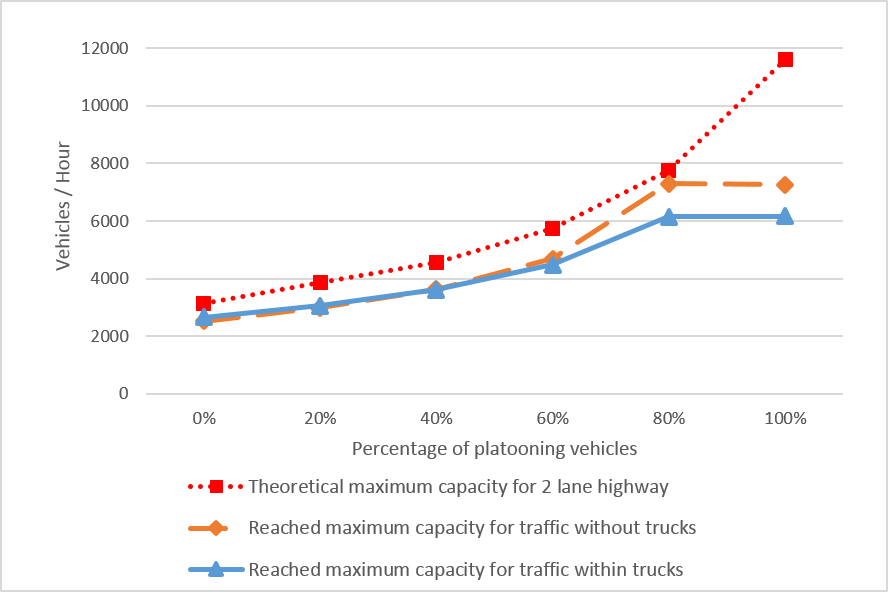
\includegraphics[width=0.82\textwidth,height=0.82\textheight,keepaspectratio]{figures/Chapter_5/5_E3_maxCap.png}
\centering
\protect\caption[Maximum capacity of two-lane highway of Theoretical example, real traffic without truck and real traffic with trucks]{\label{fig:5_3-4}Maximum capacity of two-lane highway of Theoretical example, real traffic without truck and real traffic with trucks - capacity measured only for 0\%, 20\%, 40\%, 60\%, 80\%, 100\% platooning vehicles, so as to be more visual the line connecting measured data was added.}
\end{figure}

The effect of vehicle \textit{speed dispersion} results in a reduction of efficiency of platooning concept. It is caused by slowing down of each lane by the slower vehicles. Truck traffic also negatively effects the effectiveness of platooning on maximum capacity. The reason of that is the composition of traffic, 35\% of all traffic are trucks which occupy the slowest lane and their maximum speed is 25 m/s. It can be said they make the lane unusable for platoons of passenger vehicles.














\section[Experiment \#4: Maximum capacity of three-lane highway with real traffic conditions of the Czech Republic]{Experiment \#4: Maximum capacity of three-lane highway with real traffic conditions of the Czech Republic\sectionmark{Experiment \#4...}}
\sectionmark{Experiment \#4...}

This experiment is very similar to Experiment \#3. With the same conditions we run the simulation of highway of length 5 km for 15 minutes to find out, how the traffic would behave for different percentage of platooning vehicles. 

We expected that, according to the results from Experiment \#2 and the table \ref{tab:5_2-1}, the maximum capacity of three-lane highway with traffic without trucks is proportionally smaller than theoretical maximum capacity. But for traffic with trucks we expected increasing of maximum capacity. According to 35\% representation of trucks in the traffic, the lane on the very right serves for  truck traffic and the other  two left lanes can be fully used for platooning passenger vehicles.



\subsection*{Simulator setting for the test}
\begin{itemize}
\item Average speed: 34 m/s
\item Speed dispersion: 3 m/s
\item Length of platoon: 2-6
\item Number of lanes:  3
\item Platooning vehicles ratio: 0\%, 20\%, 40\%, 60\%, 80\%, 100\%
\item Generation limit: false
\item Generate trucks: false, true
\item Percentage of passenger vehicles in traffic: 65\%
\item Overtaking: Snake type
\end{itemize}



\subsection*{Experiment results}
We did simulations with traffic in three-lane highway without truck traffic (see maximum reached capacity during time in Figure \ref{fig:5_4-1}) and with included truck traffic (See level of maximum reached capacity during time in Figure \ref{fig:5_4-2}). The simulations show very similar trend of results such as Experiment \#3.


\begin{figure}[ph]
\centering
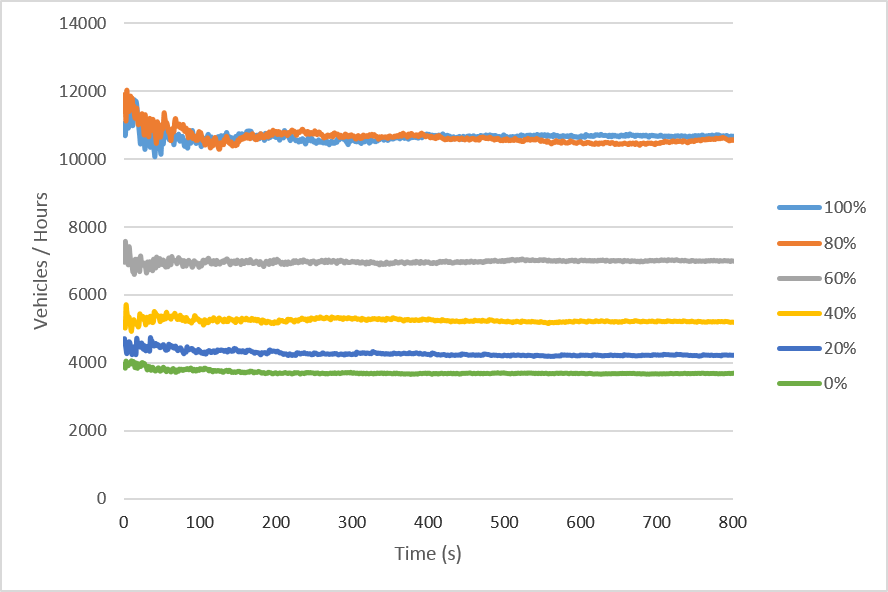
\includegraphics[width=0.82\textwidth,height=0.82\textheight,keepaspectratio]{figures/Chapter_5/5_3l_NT_maxCap.png}
\centering
\protect\caption[Maximum capacity of three-lane highway and real traffic conditions without trucks]{\label{fig:5_4-1}Maximum capacity of three-lane highway and real traffic conditions without trucks}
\end{figure}

\begin{figure}[ph]
\centering
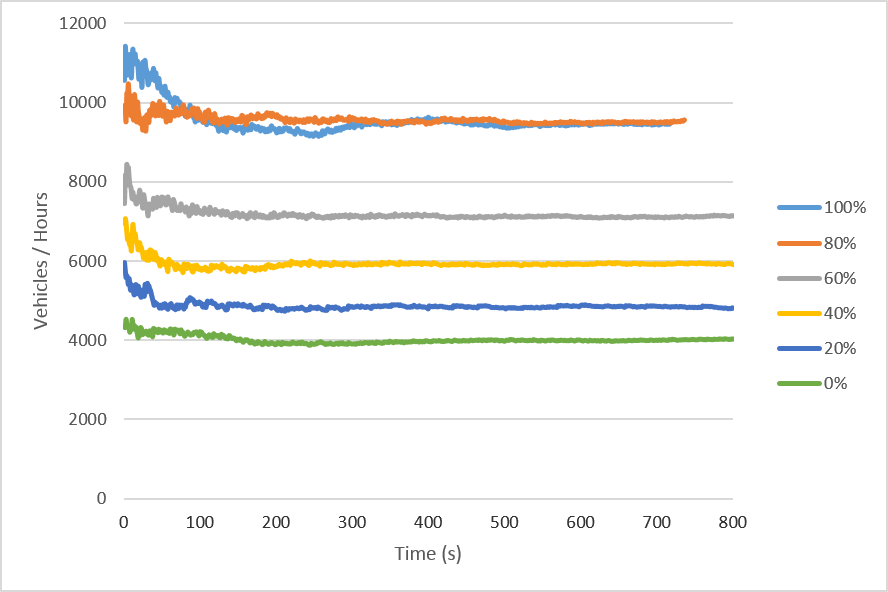
\includegraphics[width=0.82\textwidth,height=0.82\textheight,keepaspectratio]{figures/Chapter_5/5_3l_T_maxCap.png}
\centering
\protect\caption[Maximum capacity of three-lane highway and real traffic conditions with trucks]{\label{fig:5_4-2}Maximum capacity of three-lane highway and real traffic conditions with trucks}
\end{figure}


Comparison of ratio between theoretical maximum values and our reached ones in Table \ref{tab:5_4-1} and Table \ref{tab:5_3-1} of previous Experiment \#3 showed that platooning has positive effect on traffic with trucks in three-lane highway and traffic without trucks in two-lane highway. We could see during each simulation that the slowest lane of three-lane highway was used only for truck traffic.

\begin{table}[ph]
\begin{centering}
\begin{tabular}{|c|c|c|c|c|c|c|}
\hline 
 ... / Platooning \% &	0\% &	20\% &	40\% &	60\% &	80\% &	100\%\tabularnewline
\hline 
Theoretical maximum &	4 725 &	5 793 &	6 840 &	8622 &	11 634 &	17 433
\tabularnewline
 capacity for 3 lane highway & & & & & &\tabularnewline
\hline 
Reached maximum capacity & 3 661 &	4 230 &	5 219 &	6 993 &	10 478 &	10 677
\tabularnewline
for traffic without trucks & & & & & &\tabularnewline
\hline 
Ratio Theoretical maximum & & & & & &\tabularnewline
capacity / Reached maximum & 77.49\% &	73.01\% &	76.30\% &	81.11\% &	90.06\% &	61.24\%\tabularnewline
capacity without trucks & & & & & &\tabularnewline
\hline 
Reached maximum capacity & 4 001 &	4 845 &	5 920 &	7 108 &	9 501 &	9 448\tabularnewline
for traffic with trucks & & & & & &\tabularnewline
\hline 
Ratio Theoretical maximum & & & & & &\tabularnewline
capacity / Reached maximum & 84.68\% &	83.63\% &	86.56\% &	82.43\% &	81.67\% &	54.20\%\tabularnewline
capacity with trucks & & & & & &\tabularnewline
\hline 
\end{tabular}
\centering
\protect\caption{\label{tab:5_4-1}Reached maximum capacities of three-lane highway and their comparison to theoretical maximum 3 lane highway}
\end{centering}
\end{table}

\begin{figure}[ph]
\centering
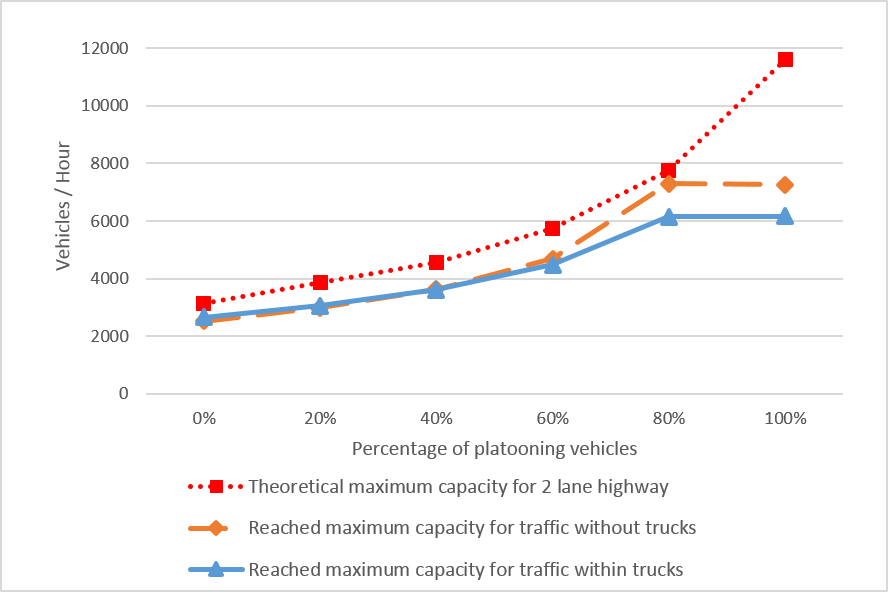
\includegraphics[width=0.82\textwidth,height=0.82\textheight,keepaspectratio]{figures/Chapter_5/5_2lane_maxCap.png}
\centering
\protect\caption[Maximum capacity of three-lane highway of Theoretical example, real traffic without truck and real traffic with trucks]{\label{fig:5_4-3}Maximum capacity of three-lane highway of Theoretical example, real traffic without truck and real traffic with trucks - capacity measured only for 0\%, 20\%, 40\%, 60\%, 80\%, 100\% platooning vehicles, so as to be more visual the line connecting measured data was added.}
\end{figure}

We measured average speed of passenger vehicles which can be seen in Figure \ref{fig:5_4-4}. Both experiments \#3 and \#4 show the relation between percentage of platooning vehicles and average speed in maximum usage of highway.  There is trend, that with increasing percentage of platooning vehicles the average speed is decreasing in time. The reason of that is studied in next Chapter 6.

\begin{figure}[!htbp]
\centering
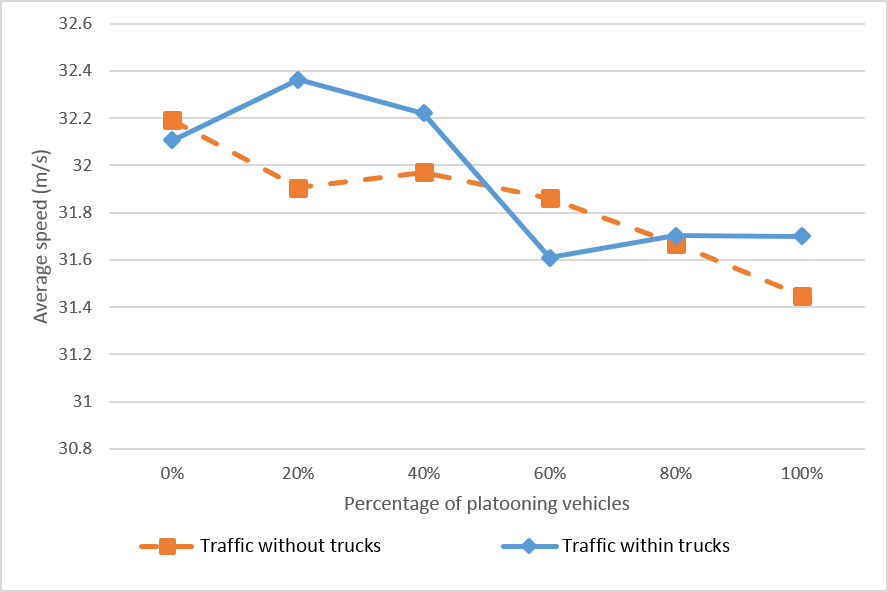
\includegraphics[width=0.82\textwidth,height=0.82\textheight,keepaspectratio]{figures/Chapter_5/5_E4_averageSpeed.png}
\centering
\protect\caption[Average speed of traffic without and with trucks in three-lane highway]{\label{fig:5_4-4}Average speed of traffic without and with trucks in three-lane highway - average speed measured after stabilization of traffic and only for 0\%, 20\%, 40\%, 60\%, 80\%, 100\% platooning vehicles, so as to be more visual the line connecting measured data was added.}
\end{figure}















\newpage
\section[Experiment \#5: Effect of platooning concept on Traffic model \#1 ]{Experiment \#5: Effect of platooning concept on Traffic model \#1\sectionmark{Experiment \#5...}}
\sectionmark{Experiment \#5...}

We used platooning concept on real traffic situation of Czech highway. The experiment setting is based on parameters of traffic model \#1 in Chapter 2 (three-lane highway). Based on information from previous Experiment \#4 we knew that maximum capacity of three-lane highway without platooning concept is cca 3700 vehicles per hour (Table \ref{tab:5_4-1}). Traffic model \#1 supposes density of vehicles 3200 vehicles per hour, so we can expect that platoons make the highway more „open“ and could increase average speed of passenger vehicles.

We also wanted to see how the platooning concept influences the traffic model \#1 with double level of traffic density, 6400 vehicles per hour. Based on the previous experiments, we knew that this capacity cannot be reached without higher level of percentage of platoon vehicles.



\subsection*{Simulator setting for the test}

Settings of Traffic model \#1.
\begin{itemize}
\item Average speed: 34 m/s
\item Speed dispersion: 3 m/s
\item Length of platoon: 2-6
\item Number of lanes:  3
\item Platooning vehicles ratio: 0\%, 20\%, 40\%, 60\%, 80\%, 100\%
\item Generation limit: 3200 vehicles / hour, 6400 vehicles / hour
\item Generate trucks: true
\item Percentage of passenger vehicles in traffic: 67\%
\item Overtaking: Snake type
\end{itemize}




\subsection*{Experiment results}

From this test which corresponds to traffic model \#1 and from the Figure \ref{fig:5_5-1} we could see that average speed of passenger vehicles is reduced to level 32.8 m/s for 0\% platooning vehicles . It is caused by high density of vehicles which is close to the maximum capacity of three-lane highway. And for for 100\% platooning vehicles the average speed reached value  34.3 m/s. The Figure \ref{fig:5_5-1} also shows a positive effect of platooning on average speed in simulated situation based on real traffic parameters.

We also simulated Traffic model \#1 with double traffic. The desired traffic density was reached between 40\% and 60\% platooning vehicles as can be seen in Figure \ref{fig:5_5-2}. In Figure \ref{fig:5_5-1} the positive effect of platooning on average speed can be also seen.




\begin{figure}[ht]
\centering
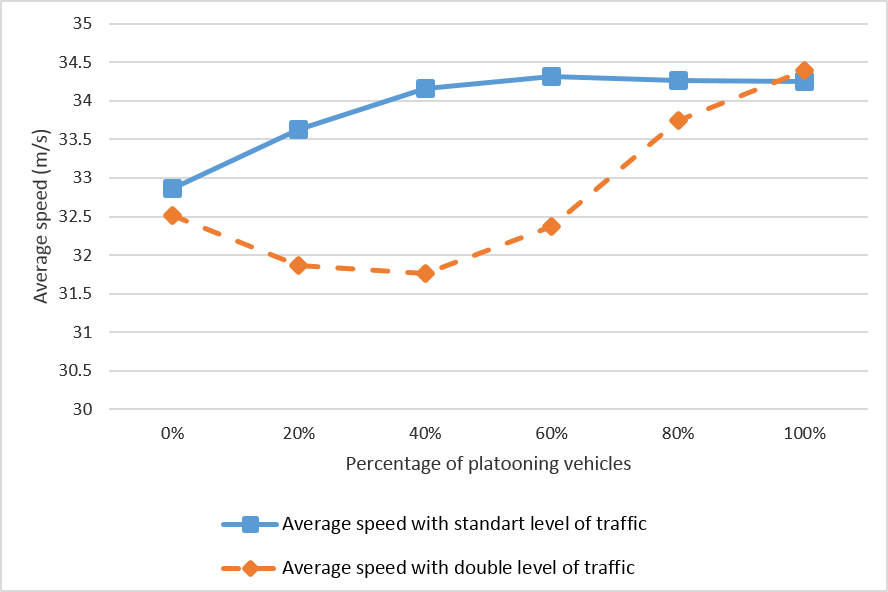
\includegraphics[width=0.82\textwidth,height=0.80\textheight,keepaspectratio]{figures/Chapter_5/5_M1_avgSpeed.png}
\centering
\protect\caption[Average speed of Traffic model \#1 with standard and double level of traffic]{\label{fig:5_5-1}Average speed of Traffic model \#1 with standard and double level of traffic - average speed measured after stabilization of traffic and only for 0\%, 20\%, 40\%, 60\%, 80\%, 100\% plat. vehicles, so as to be more visual the line connecting meas. data was added.}
\end{figure}


\begin{figure}[!htbp]
\centering
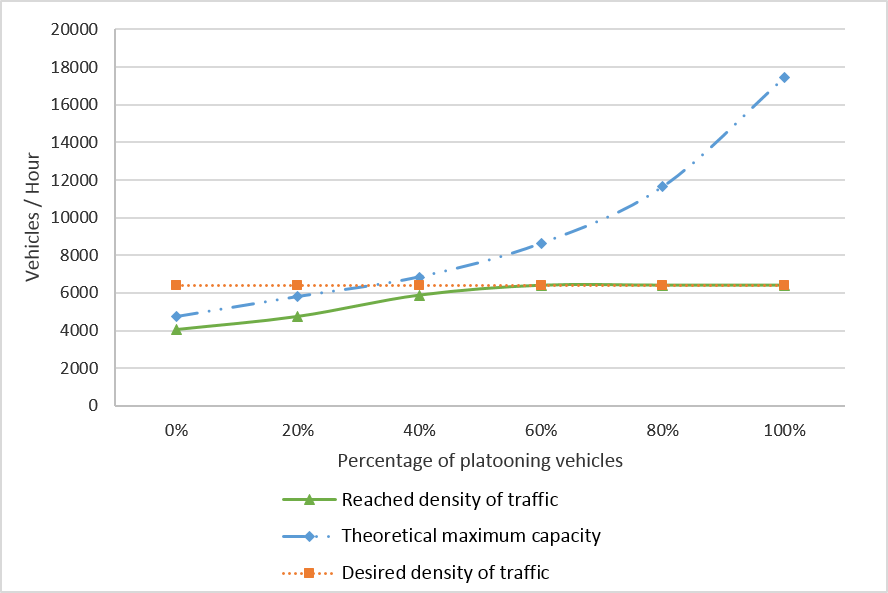
\includegraphics[width=0.82\textwidth,height=0.80\textheight,keepaspectratio]{figures/Chapter_5/5_M1D_cap.png}
\centering
\protect\caption[Reached density of Traffic model \#1 with double level of traffic for  percentage of platooning vehicles]{\label{fig:5_5-2}Reached density of Traffic model \#1 with double level of traffic for percentage of platooning vehicles - traffic density measured only for 0\%, 20\%, 40\%, 60\%, 80\%, 100\% platooning vehicles, so as to be more visual the line connecting measured data was added.}
\end{figure}

















\newpage
\section[Experiment \#6: Effect of platooning concept on Traffic Model \#2]{Experiment \#6: Effect of platooning concept on Traffic Model \#2\sectionmark{Experiment \#6...}}
\sectionmark{Experiment \#6...}


This experiment had the same assumption as Experiment \#5 but only for Traffic model \#2 (two- lane highway).



\subsection*{Simulator setting for the test}
Settings of Traffic model \#2.
\begin{itemize}
\item Average speed: 34 m/s
\item Speed dispersion: 3 m/s
\item Length of platoon: 2-6
\item Number of lanes:  2
\item Platooning vehicles ratio: 0\%, 20\%, 40\%, 60\%, 80\%, 100\%
\item Generation limit: 1650 vehicles / hour, 3300 vehicles / hour
\item Generate trucks: true
\item Percentage of passenger vehicles in traffic: 67\%
\item Overtaking: Snake type
\end{itemize}



\subsection*{Experiment results}

From this experiment of standard Traffic model \#2, in the Figure \ref{fig:5_6-1}, we could see that average speed of passenger vehicles is reduced to level 33.2 m/s for 0\% platooning vehicles. It is higher  average speed than we could see in Experiment \#5, the Figure \ref{fig:5_5-1}, but this test is two-lane highway and Experiment \#5 was three-lane highway . The Figure \ref{fig:5_6-1} also shows again a positive effect of platooning on average speed in real situation. Value of average speed is increasing with percentage of platooning vehicles, with 100\% the value with higher than 34 m/s.

Double of the capacity of Traffic model \#2 was reached between 20\% and 40\% platooning vehicles and  in Figure \ref{fig:5_6-2}  the positive effect of platooning on average speed can be also seen.


\begin{figure}[ph]
\centering
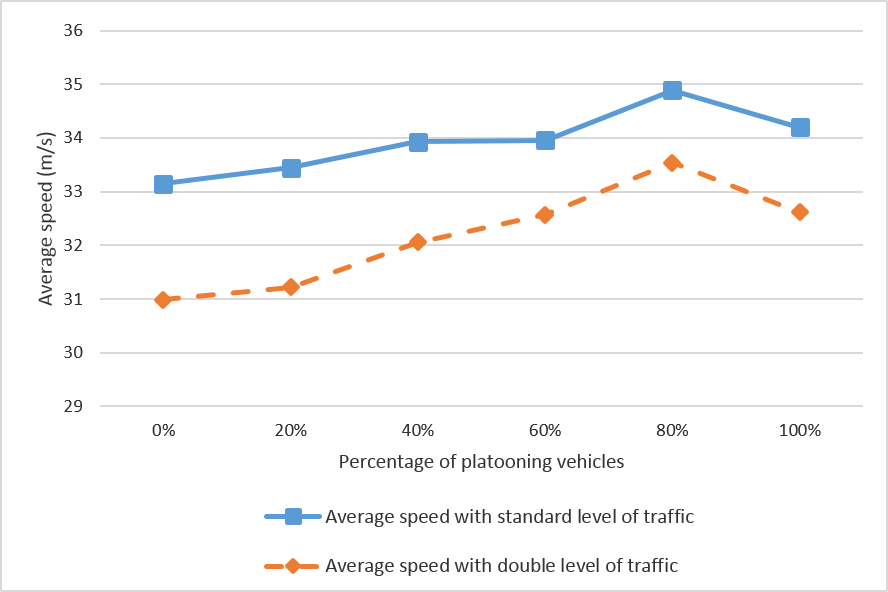
\includegraphics[width=0.82\textwidth,height=0.80\textheight,keepaspectratio]{figures/Chapter_5/5_M2_avgSpeed.png}
\centering
\protect\caption[Average speed of Traffic model \#2 with standard and double level of traffic]{\label{fig:5_6-1}Average speed of Traffic model \#2 with standard and double level of traffic - average speed measured after stabilization of traffic and only for 0\%, 20\%, 40\%, 60\%, 80\%, 100\% platooning vehicles, so as to be more visual the line connecting measured data was added.}
\end{figure}


\begin{figure}[ph]
\centering
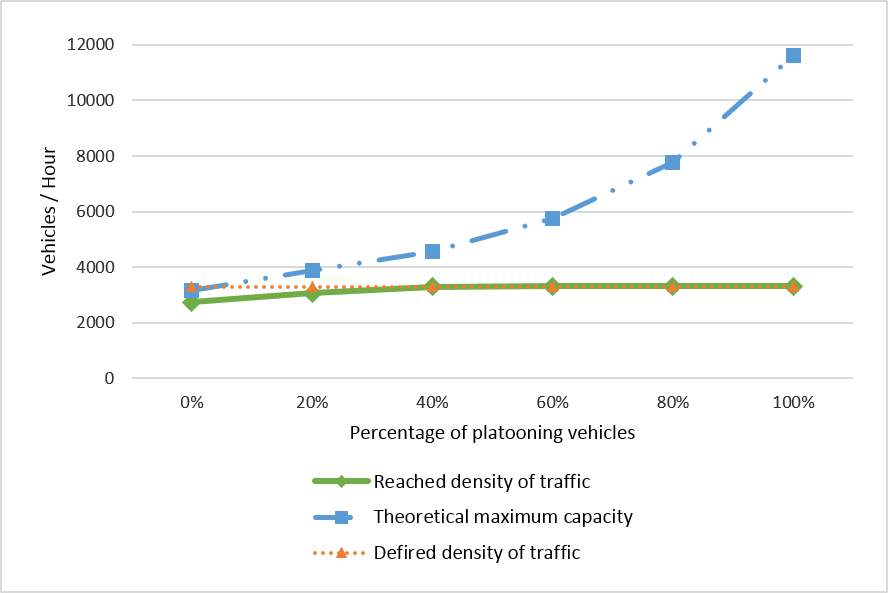
\includegraphics[width=0.82\textwidth,height=0.80\textheight,keepaspectratio]{figures/Chapter_5/5_M2D_cap.png}
\centering
\protect\caption[Reached density of Traffic model \#2 with double level of traffic for  percentage of platooning vehicles]{\label{fig:5_6-2}Reached density of Traffic model \#2 with double level of traffic for  percentage of platooning vehicles - traffic density measured only for 0\%, 20\%, 40\%, 60\%, 80\%, 100\% platooning vehicles, so as to be more visual the line connecting measured data was added.}
\end{figure} 

\chapter{Cooperative formations}

This chapter covers testing of different platooning cooperative actions – overtaking - and its effect on maximum capacity, average speed in real traffic conditions of Traffic model \#1, \#2 and number of dangerous situations of Traffic model \#1, \#2. 

For all tests in this chapter we switched off the decomposition of platoon in dangerous situation described in Section 4.2.4 for Snake overtaking type, to measure how dangerous are the non-cooperative and cooperative overtaking actions. The dangerousness is described by number of collision per hour and we evaluated it in all simulated environment, so in our case, for two or three-lane highway of length 5 km.

\section{Types of changing of lanes}

In the simulator there are programmed 3 types of overtaking and in Chapter 4 there is functionality description. In this section we did little conceptual overview of advantages and disadvantages, as well as some expected effects on a traffic.

\subsection{Snake}

Snake type of changing of lane is the easiest type of this action. It is non-cooperative action which depends only on decision of Lead vehicle of the platoon, so the lead vehicle do not any worry about the state of other following vehicles in the platoon.

Because all vehicles of platoon do the same action (changing of lane) at the same point of highway there is a risk, that the lead platoon vehicle driver does not properly estimate overtaking distance for whole platoon, it means that overtaking distance of each following vehicle in the platoon does not satisfy the safety rules. This type of overtaking action is safety for overtaking of a standing object, but not for overtaking of a moving object. The moving overtaken vehicle can get pretty close to the point, where the lead vehicles made back changing of lane from left to right lane and also each following platoon vehicle should make changing of lane. So it is necessary that each vehicle of the platoon has to evaluate possible collision all time during this operation. In order to minimize this danger there should be a such control module in each vehicle of platoon. And if it is not possible to make back changing of lane for some following platoon vehicle, then this vehicle must splits the platoon and becomes from the following vehicle into lead vehicle of newly created platoon to eliminate the collision situation.

There are still some other conceptual problems. Example of such problems is unexpected taking over the control of the following vehicle by its driver, because following platoon vehicle is managed “semi automatically by platoon”. The lead vehicle driver starts a “dangerous” overtaking or changing of lane and the following vehicle driver will respect safety rules and did not follow lead vehicle. 

If the decomposition of platoon is switched off in simulator, collisions will dramatically made the overtaken vehicle to decrease its speed. It would be reflected in simulator by decreasing of average speed.

\subsection{All at once}

It is cooperative changing of lane action which assumes reciprocal to each other knowledge of traffic situation of all platoon vehicles. As the name says the platoon can overtake only if no vehicle of platoon would not be endanger. All vehicles change the lane at same time. This changing of lane action should not finish by decomposition of platoon.

On the other hand, changing of lane All at once needs more free space for this action. Platoon of 6 vehicles with their length 4 meters and distances between vehicles 6m, need 50 meters and more of free space then overtaking action by single vehicle. It can result at deadlock between slow vehicles (trucks) in higher level of traffic density. It could decrease maximum capacity of highway and the average speed too.

\subsection{Last first}

This type of cooperative overtaking action is a hybrid between Snake type and All at once type and it consist of two steps. If lead vehicle decides about overtaking, the last following vehicle does changing of lane as first one if safety conditions are not broken. Then if it is possible all rest platoon vehicles change the lane too. If the first action, changing of line by last vehicle,  is safely done then the changing of lane by all platoon vehicles could  be done in  smaller free space. The last vehicle also “protect” rest platoon vehicles from some faster vehicles which are back in the lane. These “faster vehicles” should slow down for “short time”.

Unlike All at once overtaking, this Last first concept should increase capacity and average speed, because of easier changing of lane.






\newpage
\section[Experiment \#7: Maximum capacity of two-lane highway with real traffic and cooperative platooning]{Experiment \#7: Maximum capacity of two-lane highway with real traffic and cooperative platooning\sectionmark{Experiment \#7...}}
\sectionmark{Experiment \#7...}

According to Section 6.1 we expected little decrease of maximum capacity of highway.



\subsection*{Simulator setting for the test}
\begin{itemize}
\item Average speed: 34 m/s
\item Speed dispersion: 3 m/s
\item Length of platoon: 2-6
\item Number of lanes:  2
\item Platooning vehicles ratio: 0\%, 20\%, 40\%, 60\%, 80\%, 100\%
\item Generation limit: false
\item Generate trucks: true
\item Percentage of passenger vehicles in traffic: 67\%
\item Overtaking: Snake type, All at once type, Last fist type
\end{itemize}



\subsection*{Experiment results}

In Figure \ref{fig:6_2_2-1} there is dependency between maximum capacity of two-lane highway and percentage of platooning vehicles. This Experiment proved a negative effect of cooperative formation on maximum capacity of highway in higher level of percentage of platooning vehicles. 

For changing of lane by type All at once we supposed such result, because it is necessary to have more space for overtaking, but for Last first changing of lane we expected a little better results, but the values are smaller than type Snake.


In Figure \ref{fig:6_2_2-2} can be seen the difference of collision potential between cooperative and non-cooperative changing of lane.

\begin{figure}[!htbp]
\centering
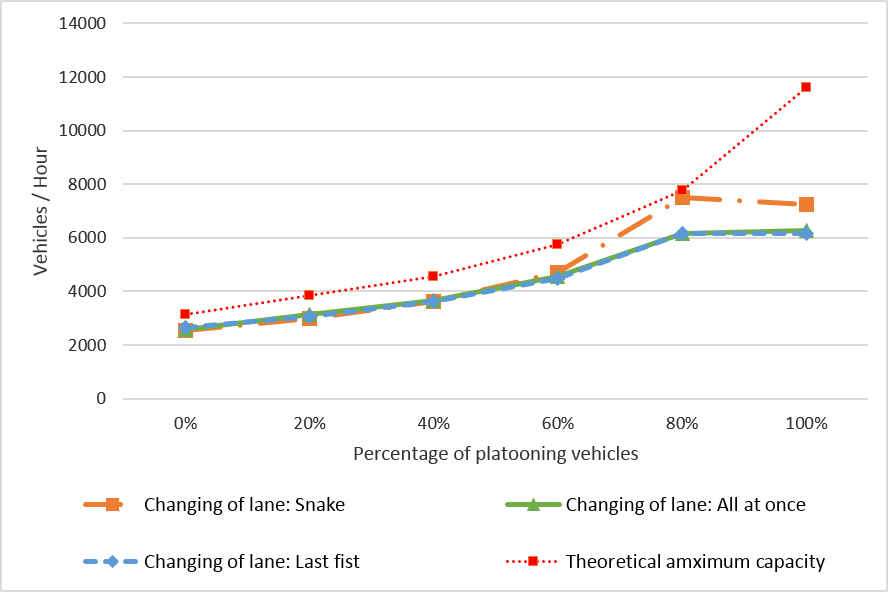
\includegraphics[width=0.82\textwidth,height=0.82\textheight,keepaspectratio]{figures/Chapter_6/6_E1_maxCap.png}
\centering
\protect\caption[Maximum capacity of two-lane highway with cooperate platoons]{\label{fig:6_2_2-1}Maximum capacity of two-lane highway with cooperative platoons - capacity measured only for 0\%, 20\%, 40\%, 60\%, 80\%, 100\% platooning vehicles, so as to be more visual the line connecting measured data was added.}
\end{figure}

\begin{figure}[!htbp]
\centering
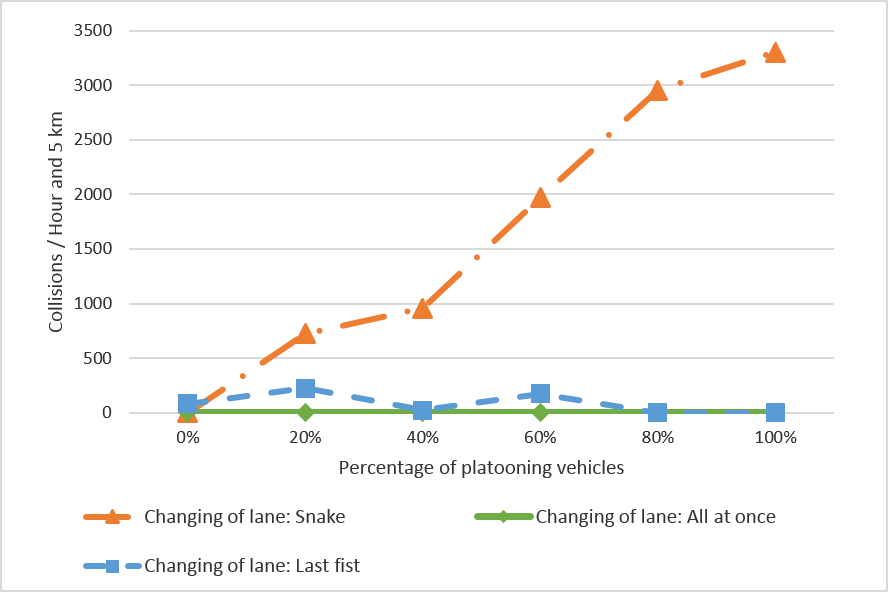
\includegraphics[width=0.82\textwidth,height=0.82\textheight,keepaspectratio]{figures/Chapter_6/6_E1_collision.png}
\centering
\protect\caption[Collisions per hour in simulated environment in simulated environment of maximum capacity of two-lane highway]{\label{fig:6_2_2-2}Collisions per hour in simulated environment in simulated environment of maximum capacity of two-lane highway - collisions measured only for 0\%, 20\%, 40\%, 60\%, 80\%, 100\% platooning vehicles, so as to be more visual the line connecting measured data was added.}
\end{figure}










\newpage
\section[Experiment \#8: Maximum capacity of three-lane highway with real traffic and cooperative platooning]{Experiment \#8: Maximum capacity of three-lane highway with real traffic and cooperative platooning\sectionmark{Experiment \#8...} }
\sectionmark{Experiment \#8...}

According to Section 6.1 we expected little decrease of maximum capacity of highway.


\subsection*{Simulator setting for the test}
\begin{itemize}
\item Average speed: 34 m/s
\item Speed dispersion: 3 m/s
\item Length of platoon: 2-6
\item Number of lanes:  3
\item Platooning vehicles ratio: 0\%, 20\%, 40\%, 60\%, 80\%, 100\%
\item Generation limit: false
\item Generate trucks: true
\item Percentage of passenger vehicles in traffic: 67\%
\item Overtaking: Snake type, All at once type, Last fist type
\end{itemize}



\subsection*{Experiment results}

In Figure \ref{fig:6_3_2-1} show us very similar results as in Experiment \#7, which proves the same negative effect of cooperative formation on maximum capacity of highway.




\begin{figure}[!htbp]
\centering
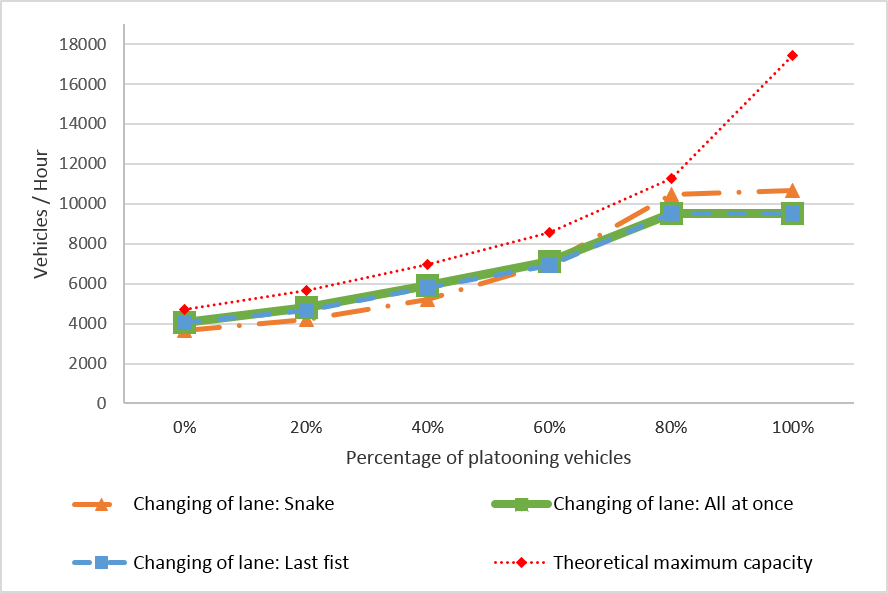
\includegraphics[width=0.82\textwidth,height=0.82\textheight,keepaspectratio]{figures/Chapter_6/6_E2_maxCap.png}
\centering
\protect\caption[Maximum capacity of three-lane highway with cooperate platoons]{\label{fig:6_3_2-1}Maximum capacity of three-lane highway with cooperate platoons - capacity measured only for 0\%, 20\%, 40\%, 60\%, 80\%, 100\% platooning vehicles, so as to be more visual the line connecting measured data was added.}
\end{figure}










\newpage
\section[Experiment \#9: Effect of cooperative platooning concept on traffic model \#1]{Experiment \#9: Effect of cooperative platooning concept on traffic model \#1\sectionmark{Experiment \#9...} }
\sectionmark{Experiment \#9...}

Overall positive effect of both cooperative and non-cooperative platooning was confirmed by previous experiments. We wanted also to test an effect of cooperative platooning on our real Traffic models.

\subsection*{Simulator setting for the test}
Settings of Traffic model \#1.
\begin{itemize}
\item Average speed: 34 m/s
\item Speed dispersion: 3 m/s
\item Length of platoon: 2-6
\item Number of lanes:  3
\item Platooning vehicles ratio: 0\%, 20\%, 40\%, 60\%, 80\%, 100\%
\item Generation limit: 3200 vehicles/hour
\item Generate trucks: true
\item Percentage of passenger vehicles in traffic: 67\%
\item Overtaking: Snake type, All at once type, Last fist type
\end{itemize}


\subsection*{Experiment results}

Based on our tests, with very similar results as in Figure \ref{fig:6_4_2-1} we were not able to confirm the assumption of increasing average speed of passenger vehicles by cooperative changing of lane in Traffic model \#1. But the cooperative approach had positive effect on safety of traffic in Traffic model \#1 (Figure \ref{fig:6_4_2-2}). The All at once changing of lane had zeros level of collisions but the unfortunately Last fist concept had some troubles. It was probably  due by a mistake in our simulator.


\begin{figure}[ph]
\centering
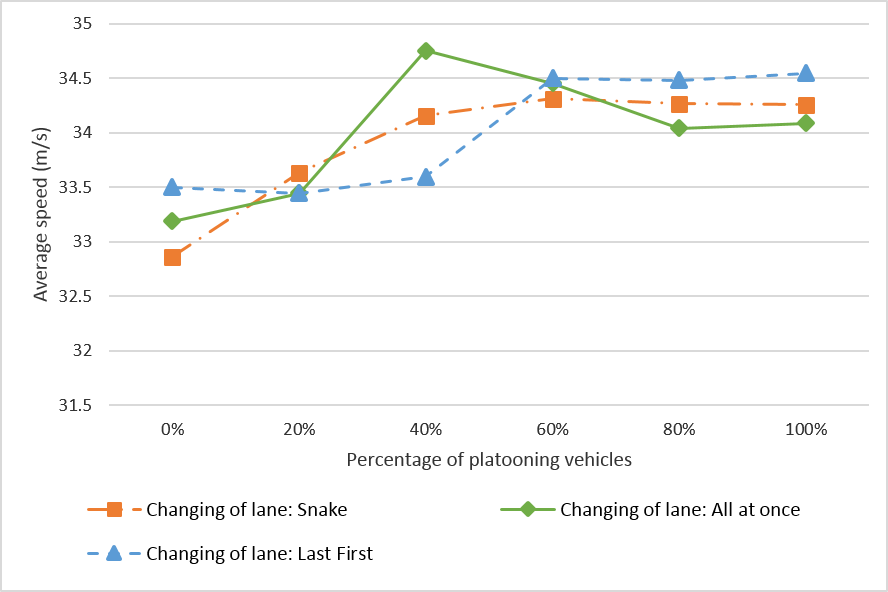
\includegraphics[width=0.82\textwidth,height=0.82\textheight,keepaspectratio]{figures/Chapter_6/6_E3_avgSpeed.png}
\centering
\protect\caption[Average speed of Traffic model \#1 with cooperative platoons]{\label{fig:6_4_2-1}Average speed of Traffic model \#1  with cooperative platoons - average speed measured after stabilization of traffic and only for 0\%, 20\%, 40\%, 60\%, 80\%, 100\% platooning vehicles, so as to be more visual the line connecting measured data was added.}
\end{figure}

\begin{figure}[!htbp]
\centering
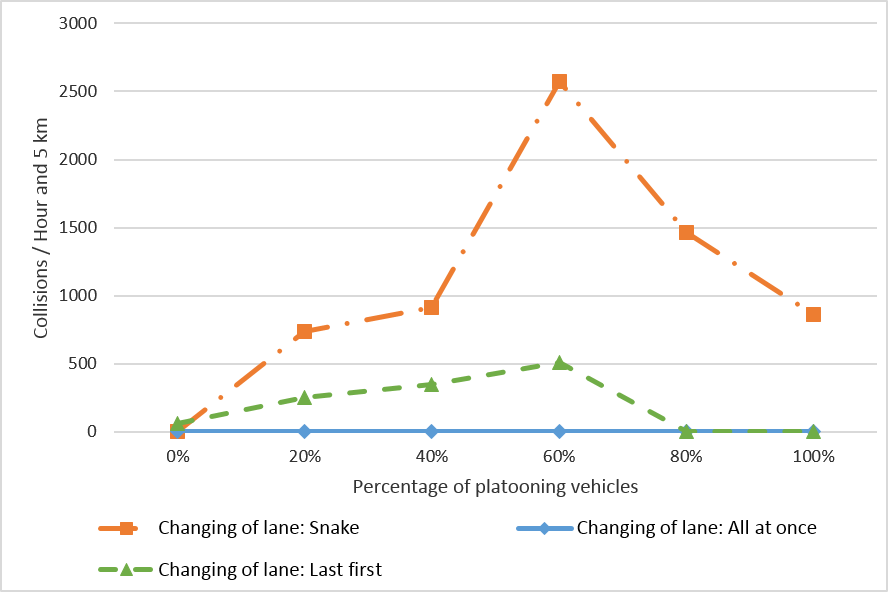
\includegraphics[width=0.82\textwidth,height=0.82\textheight,keepaspectratio]{figures/Chapter_6/6_E3_collision.png}
\centering
\protect\caption[Collisions per hour in simulated environment  of Traffic model \#1 with cooperative platoons]{\label{fig:6_4_2-2}Collisions per hour in simulated environment  of Traffic model \#1 with cooperative platoons - collisions measured only for 0\%, 20\%, 40\%, 60\%, 80\%, 100\% platooning vehicles, so as to be more visual the line connecting measured data was added.}
\end{figure}







\newpage
\section[Experiment \#10: Effect of cooperative platooning concept on traffic model \#2]{Experiment \#10: Effect of cooperative platooning concept on traffic model \#2\sectionmark{Experiment \#10...} }
\sectionmark{Experiment \#10...}

We also tested effect of cooperative changing of lane in Traffic model \#2.

\subsection*{Simulator setting for the test}
Settings of Traffic model \#2.
\begin{itemize}
\item Average speed: 34 m/s
\item Speed dispersion: 3 m/s
\item Length of platoon: 2-6
\item Number of lanes:  2
\item Platooning vehicles ratio: 0\%, 20\%, 40\%, 60\%, 80\%, 100\%
\item Generation limit: 1650 vehicles/hour
\item Generate trucks: true
\item Percentage of passenger vehicles in traffic: 67\%
\item Overtaking: Snake type, All at once type, Last fist type
\end{itemize}


\subsection*{Experiment results}

This experiment gave us some similar results as Experiment \#9 (Figure \ref{fig:6_5_2-1} and Figure \ref{fig:6_5_2-2}). We were not able to confirm expected increase of average speed, but again cooperation had positive effect on traffic safety.


\begin{figure}[ph]
\centering
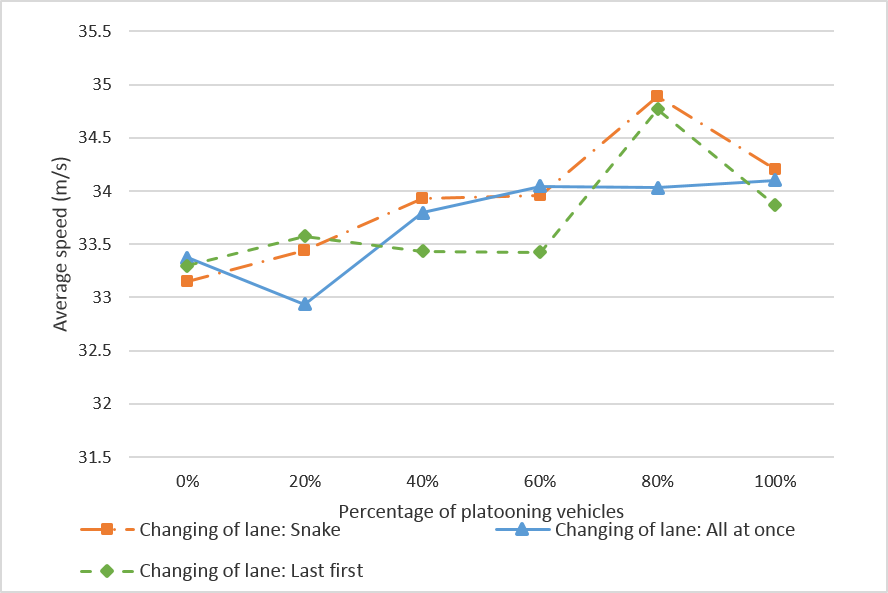
\includegraphics[width=0.82\textwidth,height=0.82\textheight,keepaspectratio]{figures/Chapter_6/6_E4_avgSpeed.png}
\centering
\protect\caption[Average speed of Traffic model \#2 with cooperative platoons]{\label{fig:6_5_2-1}Average speed of Traffic model \#2 with cooperative platoons - average speed measured after stabilization of traffic and only for 0\%, 20\%, 40\%, 60\%, 80\%, 100\% platooning vehicles, so as to be more visual the line connecting measured data was added.}
\end{figure}

\begin{figure}[ph]
\centering
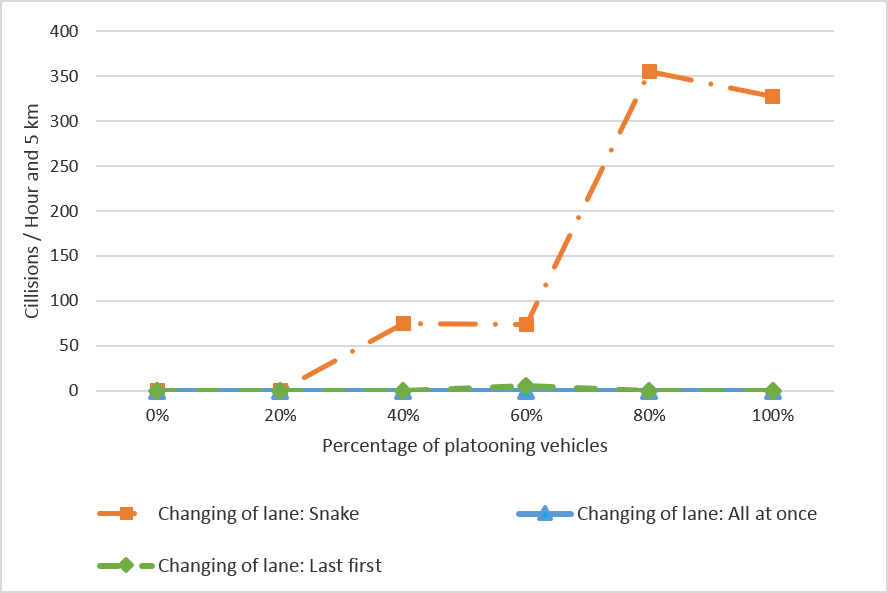
\includegraphics[width=0.82\textwidth,height=0.82\textheight,keepaspectratio]{figures/Chapter_6/6_E4_collision.png}
\centering
\protect\caption[Collisions per hour in simulated environment  of Traffic model \#2 with cooperative platoons]{\label{fig:6_5_2-2}Collisions per hour in simulated environment  of Traffic model \#2 with cooperative platoons - collisions measured only for 0\%, 20\%, 40\%, 60\%, 80\%, 100\% platooning vehicles, so as to be more visual the line connecting measured data was added.}
\end{figure}
 

\chapter{Conclusion}

Concept of platooning is known for long time, but is not still fully appreciated. We focused on overall positive effect of platooning and its potential for nowadays traffic in Czech highways from point of view of maximum capacity of highway and average speed. We did not deal with custom intern control of platoon itself, but we wanted to test cooperative approach to changing of lanes during various common action of travelling in highway such as overtaking.

For this purpose we upgraded an exist traffic simulator with many different adjustable features and we developed new module to be able to simulate platooning in highway. Result values from simulator “nearly” correspond to the theoretical model, and therefore we used it for simulation of traffic models, that represent required traffic situations. The simulated traffic experiments are based on real traffic statistic data that we gain by studying of several sources. The experiment parameters in combination with safety traffic setting gave rise of realistic traffic simulations which match a real traffic.

The experiments proved big theoretical potential of platooning for highway traffic. In same traffic composition (ration passenger vehicles and trucks), platooning concept can increase the maximum capacity of highway more than twice as it is nowadays. We also find out, that in cause application of platooning concept for actual traffic, it can increase average speed in 1-2 m/s. This positive effects were reached for 100\% platooning vehicles and were no proportional to percentage of platooning vehicles, but still there is a positive trend.

Cooperative behaviour of platoons had only small effect on maximum capacity of highway and average speed of nowadays traffic, but it dramatically decreases number of problematic situations, which endanger both platoon vehicles and the rest participants of traffic. Complexity of cooperative actions is not high but their benefit into safety of traffic is big. There is a smaller risk  of forced platoon decomposition of endanger of other vehicles.

Based on our research we could say that concept of platooning seems to be a positive step to improve our highway traffic environment. It has positive effect even on actual traffic level and also on increased number of vehicles and also on traffic safety. It can, according to global research, safe fuel and reduce amount of produced carbon dioxide.

In future steps it could be useful to test effect on traffic during day and run test based on all week data. There could be also analysed some other principles of cooperative actions such as other types of changing of lanes, clustering of platoon, etc. There is still a place to re-implement the PlatooningCenterModule to agent structure for better utilization of Alite simulator.

All requested assignment tasks were studied, done and evaluated.

\nocite{russell2002,vokrinek2013,fernandes2010}

%*****************************************************************************


%*****************************************************************************
% Seznam literatury je v samostatnem souboru reference.bib. Ten
% upravte dle vlastnich potreb, potom zpracujte (a do textu
% zapracujte) pomoci prikazu bibtex a nasledne pdflatex (nebo
% latex). Druhy z nich alespon 2x, aby se poresily odkazy.

\bibliographystyle{abbrv}
%bibliographystyle{plain}
%\bibliographystyle{psc}
{
%JZ: 11.12.2008 Kdo chce mit v techto ukazkovych odkazech take odkaz na CSTeX:
\def\CS{$\cal C\kern-0.1667em\lower.5ex\hbox{$\cal S$}\kern-0.075em $}
\bibliography{reference}
}



%*****************************************************************************
%*****************************************************************************
\appendix

\chapter{Attached CD}
The attached CD contains:

\begin{itemize}
\item PDF version of this thesis
\item The source code of the simulator - can by run by command run.exe (run.sh)
\item The data of experiments.
\end{itemize}

\section*{}


\chapter{List of used shortcuts}

\begin{description}
\item[LV] Lead vehicle
\item[FV] Following vehicle
\item[V2V] Vehicle to vehicle communication
\item[V2I] Vehicle to infrastructure communication
\end{description}
\vdots

%*****************************************************************************


\end{document}
